%\documentclass[prb, twocolumn, 12pt]{revtex4}
%nofootinbib
\documentclass[pra,twocolumn,groupedaddress,10pt]{revtex4}

\usepackage[papersize={8.5in,11in}]{geometry} % set page size in a standard way
\usepackage{amsmath}    % need for subequations
\usepackage{amsthm}     % need for theorems and definitions
\usepackage{amssymb}     % need for symbols like \varnothing
\usepackage{graphicx}   % need for figures
\usepackage{verbatim}   % useful for program listings
\usepackage{color}      % use if color is used in text
\usepackage{subfigure}  % use for side-by-side figures
\usepackage{hyperref}   % use for hypertext links, including those to external documents and URLs
\usepackage{tikz}
%\usepackage{tikz,fullpage}
\usetikzlibrary{arrows,%
                petri,%
                topaths}%
\usepackage{tkz-berge}
\usepackage{tikz-cd}
\usepackage{mathrsfs}
\usepackage{hyperref}
\usepackage{thmtools}
\usepgflibrary{shapes}
\usepackage{url}
\usepackage[stretch=10]{microtype}

%\usepackage[position=top]{subfig}


% don't need the following. simply use defaults
\setlength{\baselineskip}{16.0pt}    % 16 pt usual spacing between lines

% below float fixing from mintaka.sdsu.edu/GF/bibliog/latex/floats.html
% Alter some LaTeX defaults for better treatment of figures:
    % See p.105 of "TeX Unbound" for suggested values.
    % See pp. 199-200 of Lamport's "LaTeX" book for details.
    %   General parameters, for ALL pages:
    \renewcommand{\topfraction}{0.9}	% max fraction of floats at top
    \renewcommand{\bottomfraction}{0.8}	% max fraction of floats at bottom
    %   Parameters for TEXT pages (not float pages):
    \setcounter{topnumber}{2}
    \setcounter{bottomnumber}{2}
    \setcounter{totalnumber}{4}     % 2 may work better
    \setcounter{dbltopnumber}{2}    % for 2-column pages
    \renewcommand{\dbltopfraction}{0.9}	% fit big float above 2-col. text
    \renewcommand{\textfraction}{0.07}	% allow minimal text w. figs
    %   Parameters for FLOAT pages (not text pages):
    \renewcommand{\floatpagefraction}{0.7}	% require fuller float pages
	% N.B.: floatpagefraction MUST be less than topfraction !!
    \renewcommand{\dblfloatpagefraction}{0.7}	% require fuller float pages

	% remember to use [htp] or [htpb] for placement

% additional definitions
% from http://www.maths.tcd.ie/~dwilkins/LaTeXPrimer/Theorems.html
\newtheorem{theorem}{Theorem}[section]
\newtheorem{lemma}[theorem]{Lemma}
\newtheorem{proposition}[theorem]{Proposition}
\newtheorem{corollary}[theorem]{Corollary}

\theoremstyle{definition}
\newtheorem{defn}{Definition}[section]

% From http://tex.stackexchange.com/questions/140978/arrow-accented-with-a-dot-natural-transformation
\newcommand{\naturalto}{%
	\mathrel{\vbox{\offinterlineskip
			\mathsurround=0pt
			\ialign{\hfil##\hfil\cr
				\normalfont\scalebox{1.2}{.}\cr
				%      \noalign{\kern-.05ex}
				$\longrightarrow$\cr}
		}}%
}

%\newenvironment{proof}[1][Proof]{\begin{trivlist}
%\item[\hskip \labelsep {\bfseries #1}]}{\end{trivlist}}
%\newenvironment{definition}[1][Definition]{\begin{trivlist}
%\item[\hskip \labelsep {\bfseries #1}]}{\end{trivlist}}
%\newenvironment{example}[1][Example]{\begin{trivlist}
%\item[\hskip \labelsep {\bfseries #1}]}{\end{trivlist}}
%\newenvironment{remark}[1][Remark]{\begin{trivlist}
%\item[\hskip \labelsep {\bfseries #1}]}{\end{trivlist}}

%\newcommand{\qed}{\nobreak \ifvmode \relax \else
%      \ifdim\lastskip<1.5em \hskip-\lastskip
%      \hskip1.5em plus0em minus0.5em \fi \nobreak
%      \vrule height0.75em width0.5em depth0.25em\fi}

%

% above is the preamble

\begin{document}

\title{Identity Architecture of Living Systems}
\author{S. Kasivajhula}
%\email{sid[at]drym.com}
%\noaffiliation
\affiliation{sid@drym.org}
%\date{\today}

\begin{abstract}

``Identity architecture shows us what things ultimately are, and how they come together. It seems that Siddhartha Gautama (the Buddha), anticipating the essence of the present work by over two thousand years, told us what that thing is that they come together as. Awareness of that thing is the experience of Nirvana -- enlightenment -- the freedom from the cycle of birth and rebirth.''

A tree-based model of identity possessing fractal properties is developed. The model is grounded in the notion of an ``identity context'' which is related to the idea of a Grothendieck Universe in set theory. A natural basis for formal undecidability is introduced, with implications for the limits of empirical science. The model is applied to privacy, the brain, economics and government, intellectual property, and to natural phenomena. Religious traditions are also addressed.

\end{abstract}

\maketitle


\section{Introduction} \label{sec:introduction}
% A Case of Identity

An ocean of sensation commences experience. This soon gives way to a calmer sea of feeling, to undulating shapes and waves of sound. Forms move, sounds ebb and flow, and other feelings move with them. Utterances gradually coalesce into words, shapes to entities, feelings differentiate into touch, taste, smell, sound, and sight. And these grow to constitute more complex models that define a tractable world of experience which, in time, gives rise to our humanity.

Along the way, we encounter others like us. Entities, that is, for which the models we develop inescapably apply equally to ourselves. As communities, we then develop models of the universe of our collective experience, and we mould this universe in ways conforming to those models. These new models are much the same as the primordial ones, but a notable feature of this collective context is that it is the one in which our conception of ``self'' is useful.

Within this realm, as part of our continuing imperative to make sense of our experience, we assign names to things, and to people. Names correspond to models, and with a sufficiently rich taxonomy we are able to characterize most of the things that we encounter. In other words we ascribe to people and things \textit{identity}, and these identities define the universe of our experience.

Identity is ultimately the only reality we know, and in the present manuscript we will attempt to establish its nature.

\subsection{Motivating Examples} \label{sec:motexa}

To motivate some of the ensuing discussion, let's consider the following (contrived) thought experiment: Voldemort is a failed Dark Lord now attempting to make a living as the town baker in a small town. He will serve all who visit his bakery except muggles. Unfortunately for Voldemort, in this little town the entire population is muggle, a fact he is as yet unaware of. Additionally, the townsfolk practice an obscure religion wherein engaging in the act of baking is forbidden. Furthermore, if they were to learn the ideological views of the baker, they would in all likelihood have him exiled.

It is apparent that as things stand, Voldemort cannot make an honest living, and the townsfolk cannot have their daily bread. There is a way out, however, and it is for the residents to withhold their status as muggles in their transactions with the baker, and for Voldemort likewise to be discreet about his ideological beliefs that have little to do with his ability to bake. In this arrangement, the town would have a competent baker, and Voldemort can be a contributing member of society despite his misguided beliefs -- an optimal result within the specified scope of the experiment.

The point to note here is that perfect fidelity of identity is oftentimes less optimal than (and merely a limiting case of) selective fidelity of identity. Taking this observation as a clue, let us develop intuition in a more familiar setting: user identity on the internet.

Traditionally in human societies, people have one official name, and this name is effective enough at characterizing an individual that there's never really been much of a need to question this basic fact of life. Some variant of ``What is your name?'' starts practically every new interaction on the planet, with the full expectation on the part of the asker of one absolute answer. The reason one identity is such an effective model for people is that cause and effect, which is ultimately what models are meant to describe, have in this case historically (usually) been localized within a single entity (``person'') that we can perceive directly with our senses.

Now with the advent of telecommunications and especially the internet, that is starting to change dramatically. Cause and effect are often separated by vast (and ``unknowable'') distances, and interactions can occur across such widely varying contexts that modeling people by a single identity is increasingly an almost arbitrary choice, and certainly no longer as effective as it once was. Indeed, although in the real world we've always employed this model to characterize others, it's rarely the one that we've assumed ourselves. People assume different identities all the time, though they may not always be aware of it (different identities employed in work and in social contexts is one of the more obvious examples). Yet by force of habit we persist in this approach of enforcing a single identity where a multitude may be a more effective model.

Finally, we note that identity applies to much more than just human interactions. Anything in the universe can be said to possess identity by definition, and so a characterization of identity itself must apply to all such things and interactions.

\subsection{Conception of a Model of Identity} \label{sec:conmodide}

Let us first, by consulting our intuition, make some observations on the nature of identity. Since we ascribe identity to every ``thing'' in our experience, we can for now consider identity as equivalent to ``thing'' (though in defining these precisely later, we will draw a distinction between them). As such, we may make the following observations:

\begin{enumerate}
	\item As motivated previously, everything in our experience is an identity.
	\item We are ourselves identities.
	\item A single identity is able to act through multiple identities (e.g. Clark Kent and Superman).
	\item Multiple identities are able to constitute a single identity (e.g. many players constitute a sports team).
	\item It is possible, in principle, to act anonymously.
\end{enumerate}

With the above properties in mind, we begin our investigation by examining several high-level structures in terms of their ability to satisfy our requirements.

\section{Topological Structure} \label{sec:topstr}

The core underlying structure we consider is a (directed) \textit{tree}. Each node in this tree represents an identity, and edges between two nodes represent constituency. That is, $A \twoheadrightarrow B$ represents that $A$ constitutes $B$. Note that, in order to have a truly general model, every identity is to be considered qualitatively equivalent to any other identity. Within this paradigm, we explore a few variations and assess them with regard to the aforementioned properties.

\subsection{Arborescence} \label{sec:arborescence}

\begin{figure}[htp]
\centering
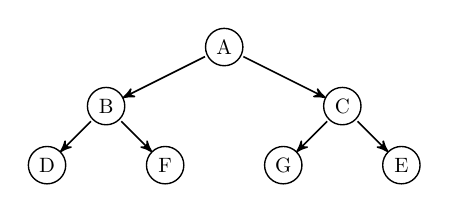
\begin{tikzpicture}[scale=0.75,transform shape]
  \tikzstyle{LabelStyle}=[fill=white,sloped]
%  \tikzstyle{EdgeStyle}=[bend left]
  \Vertex[x=0,y=0,LabelOut=false]{A}
  \Vertex[x=-2,y=-1]{B}
  \Vertex[x=2,y=-1]{C}
  \Vertex[x=-3,y=-2]{D}
  \Vertex[x=3,y=-2]{E}
  \Vertex[x=-1,y=-2]{F}
  \Vertex[x=1,y=-2]{G}
  \tikzstyle{EdgeStyle}=[post]
  \Edge[](A)(B)
  \Edge[](A)(C)
  \Edge[](B)(D)
  \Edge[](C)(E)
  \Edge[](B)(F)
  \Edge[](C)(G)
%  \Edge[label=$$](K)(F)
\end{tikzpicture}
\caption{\label{fig:arborescence}Arborescence}
\end{figure}

The arborescence\cite{arborescence} is a simple tree structure defined by having exactly one directed path from the root node to every other node in the tree. It supports each node having a number of children which may themselves have a number of children. This expresses the property of a single identity (the parent node) being able to act through multiple identities (the child nodes). Note also that, as alluded to earlier, each child node is itself an identity, qualitatively equivalent to the parent identity in every way. Therefore, this identity representation could extend an arbitrary number of levels, endlessly bifurcating all the way down.

\subsection{Polytree} \label{sec:polytree}

\begin{figure}[htp]
\centering
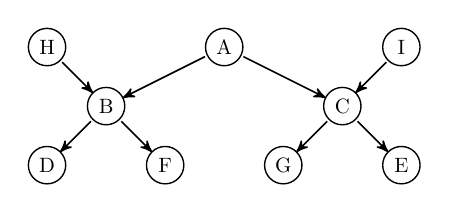
\begin{tikzpicture}[scale=0.75,transform shape]
  \tikzstyle{LabelStyle}=[fill=white,sloped]
%  \tikzstyle{EdgeStyle}=[bend left]
  \Vertex[x=0,y=0,LabelOut=false]{A}
  \Vertex[x=-2,y=-1]{B}
  \Vertex[x=2,y=-1]{C}
  \Vertex[x=-3,y=-2]{D}
  \Vertex[x=3,y=-2]{E}
  \Vertex[x=-1,y=-2]{F}
  \Vertex[x=1,y=-2]{G}
  \Vertex[x=-3,y=0]{H}
  \Vertex[x=3,y=0]{I}
  \tikzstyle{EdgeStyle}=[post]
  \Edge[](A)(B)
  \Edge[](A)(C)
  \Edge[](B)(D)
  \Edge[](C)(E)
  \Edge[](B)(F)
  \Edge[](C)(G)
  \Edge[](H)(B)
  \Edge[](I)(C)
%  \Edge[label=$$](K)(F)
\end{tikzpicture}
\caption{\label{fig:polytree}Polytree}
\end{figure}

The polytree\cite{polytree} is a more general model than the arborescence and allows a node to have multiple parents. This expresses the property of an identity being comprised by multiple identities. We call such an identity a \textit{hive identity} (a relative term) or a \textit{compound identity}. Human institutions such as marriage, nations, and corporations are such identities. Ant colonies, bee hives, starling murmurations are such identities. So in fact are physical atoms, chemical molecules, and living cells. % "chimera identity," "polytree identity" as alternative terms that are more apt / less connoted in different contexts?

\subsection{Multitree} \label{sec:multitree}

\begin{figure}[htp]
\centering
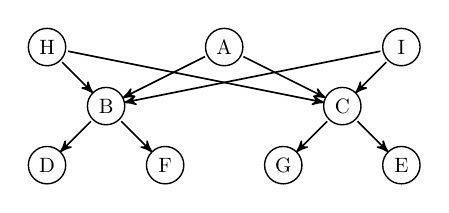
\begin{tikzpicture}[scale=0.75,transform shape]
  \tikzstyle{LabelStyle}=[fill=white,sloped]
%  \tikzstyle{EdgeStyle}=[bend left]
  \Vertex[x=0,y=0,LabelOut=false]{A}
  \Vertex[x=-2,y=-1]{B}
  \Vertex[x=2,y=-1]{C}
  \Vertex[x=-3,y=-2]{D}
  \Vertex[x=3,y=-2]{E}
  \Vertex[x=-1,y=-2]{F}
  \Vertex[x=1,y=-2]{G}
  \Vertex[x=-3,y=0]{H}
  \Vertex[x=3,y=0]{I}
  \tikzstyle{EdgeStyle}=[post]
  \Edge[](A)(B)
  \Edge[](A)(C)
  \Edge[](B)(D)
  \Edge[](C)(E)
  \Edge[](B)(F)
  \Edge[](C)(G)
  \Edge[](H)(B)
  \Edge[](I)(C)
  \Edge[](H)(C)
  \Edge[](I)(B)
%  \Edge[label=$$](K)(F)
\end{tikzpicture}
\caption{\label{fig:multitree}Multitree}
\end{figure}

The multitree\cite{multitree} is a strengthening of the polytree, possessing only the constraint that no node can have parents that have a common ancestor, i.e. that there can be no set of nodes that form a ``diamond'' in the tree. This model expresses the ability of identities to form different child identities with the same parents. For example, two people can be friends as well as colleagues. As another example, the same set of chemical elements can form two different molecules, or isomers.

\subsection{``Identitree''} \label{sec:identitree}

\begin{figure}[htp]
\centering
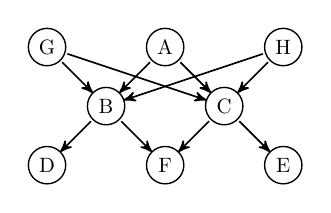
\begin{tikzpicture}[scale=0.75,transform shape]
  \tikzstyle{LabelStyle}=[fill=white,sloped]
%  \tikzstyle{EdgeStyle}=[bend left]
  \Vertex[x=0,y=0,LabelOut=false]{A}
  \Vertex[x=-1,y=-1]{B}
  \Vertex[x=1,y=-1]{C}
  \Vertex[x=-2,y=-2]{D}
  \Vertex[x=2,y=-2]{E}
  \Vertex[x=0,y=-2]{F}
  \Vertex[x=-2,y=0]{G}
  \Vertex[x=2,y=0]{H}
  \tikzstyle{EdgeStyle}=[post]
  \Edge[](A)(B)
  \Edge[](A)(C)
  \Edge[](G)(B)
  \Edge[](H)(C)
  \Edge[](B)(D)
  \Edge[](C)(E)
  \Edge[](B)(F)
  \Edge[](C)(F)
  \Edge[](G)(C)
  \Edge[](H)(B)
%  \Edge[label=$$](K)(F)
\end{tikzpicture}
\caption{\label{fig:identitree}Identitree}
\end{figure}

The identitree is a generalization of the multitree which eliminates the ``no-diamonds'' constraint. This enables identities that have common ancestors to unite. It may seem unclear why this sort of union would be needed, but consider that in the multitree model, two identities with only a single common ancestor, however distant, would be unable to unite. The identitree enables this union (which, as a clarification, does not refer to a biological relationship but a conceptual one).

\subsection{``Bodhitree''} \label{sec:bodhitree}

\begin{figure}[htp]
\centering
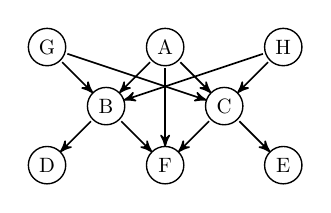
\begin{tikzpicture}[scale=0.75,transform shape]
  \tikzstyle{LabelStyle}=[fill=white,sloped]
%  \tikzstyle{EdgeStyle}=[bend left]
  \Vertex[x=0,y=0,LabelOut=false]{A}
  \Vertex[x=-1,y=-1]{B}
  \Vertex[x=1,y=-1]{C}
  \Vertex[x=-2,y=-2]{D}
  \Vertex[x=2,y=-2]{E}
  \Vertex[x=-2,y=0]{G}
  \Vertex[x=2,y=0]{H}
  \Vertex[x=0,y=-2]{F}
  \tikzstyle{EdgeStyle}=[post]
  \Edge[](A)(B)
  \Edge[](A)(C)
  \Edge[](G)(B)
  \Edge[](H)(C)
  \Edge[](B)(D)
  \Edge[](C)(E)
  \Edge[](B)(F)
  \Edge[](C)(F)
  \Edge[](G)(C)
  \Edge[](H)(B)
  \Edge[](A)(F)
%  \Edge[label=$$](K)(F)
\end{tikzpicture}
\caption{\label{fig:bodhitree}Bodhitree}
\end{figure}

The only restriction in the identitree model is that an identity cannot unite with an ancestor node. The removal of this restriction results in the ``bodhitree,'' which it can be shown is equivalent to an acyclic graph\footnote{While structurally the bodhitree is equivalent to an acyclic graph, in application the former has an implicit notion of causality, and so, as a convention, all edges flow in a particular direction to depict this (of course, there could be alternate depictions that capture this). In an acyclic graph, by contrast, there is no inherent preferred directionality.}. The ability to unite with an ancestor node seems of questionable value, but consider that in the other models with such a restriction in place, descendants are distinguished in the context of ancestors, violating our requirement for all identities to be qualitatively equivalent. We will return to this after further elaborating the mathematical model for identity. Let us first formalize the above development in precise definitions. Note that the bodhitree/acyclic graph is the most general model, with each preceding one above being a further specialization.

\begin{defn}
	A \emph{graph}\footnote{We will assume graphs are directed unless otherwise specified. Since undirected graphs may be modeled by directed graphs by treating edges as the unordered pair of directed edges $\{(u,v),(v,u)\}$\cite{chartrand}, directed graphs may be seen as a more general model, which motivates our choice of terminology.} $\Gamma$ is an ordered pair $(V, E)$ consisting of a finite nonempty set $V$ together with an irreflexive relation $E$ \cite{chartrand}. The elements of $V$ are called \emph{vertices}, or \emph{nodes}, and the elements of $E$ are ordered pairs of vertices called \emph{edges}. A (directed) sequence of linked edges connecting one vertex to another is called a \emph{path}.
	\begin{equation}
		\begin{split}
			\Gamma &= (V, E) \text{, where} \\
			V &\neq \varnothing \text{, and } E \subset V \times V \mid \\
			(u,v) \in E &\implies (v,u) \notin E \text{, and} \\
			(u,u) &\notin E \,\, \forall u \in V .
		\end{split}
		\nonumber
	\end{equation}
\end{defn}

\begin{defn}
	An \emph{acyclic graph}, or \emph{bodhitree}, is a graph such that $E$ does not contain a path from some vertex $u$ to itself.
\end{defn}

\begin{defn}
	An \emph{identitree} is a bodhitree such that if $(u, v) \in E$, then there is no path in $E - \left\{\left(u, v\right)\right\}$ originating at $u$ and terminating at $v$.
\end{defn}

\begin{defn}
	A \emph{multitree} is a bodhitree such that for any vertices $u, v \in V$, if a path exists between them then it is unique. Any multitree is also an identitree.
\end{defn}

\begin{defn}
	A \emph{polytree} is a bodhitree such that for any vertices $u, v \in V$, there is a unique undirected path (i.e. ignoring the ordering on the edges) between them. Any polytree is also a multitree.
\end{defn}

\begin{defn}
	An \emph{arborescence} is a polytree containing a least element in $V$ (``root'' vertex) with respect to the natural ordering on edges.
\end{defn}

\section{Mathematical Model} \label{sec:matmod}

\subsection{Foundations} \label{sec:foundations}

The models above characterize our high-level intuitions of the behavior of identity. Now we develop a mathematical foundation on which to base further development of the model.

Let's collect some observations, following which we'll develop the model:

\begin{enumerate}
	\item Identities must exist ``somewhere,'' i.e. within some ``context'' whose nature is to be elaborated.
	\item Since identities ought to be a universal model, it follows that anything that can be considered to ``exist'' in some context must be an identity in that context.
	\item All identities are qualitatively equivalent (and together with intuitions discussed earlier this appears to imply the bodhitree model above).
\end{enumerate}

Due to the fractal nature of identity architecture, the definitions below may sometimes reference ideas that have not yet been defined, and which are then defined later. This apparent circularity can be resolved by imagining that at the level of each definition, the referenced concepts are either at a ``lower'' or ``higher'' level as the case may be, and as such are assumed to simply have been provided beforehand, similar to the case of set theory where the elements of sets are themselves sets.

\begin{defn}[Identity Context] \label{def:idecon}
	An \emph{identity context}, or simply \emph{context}, is a universe $\mathcal{W}$ of identities (which for now can be thought of as sets) such that:
	\begin{itemize}
		\item There exists an identity with no ancestors: $\exists \varnothing_W \in \mathcal{W}$ (\emph{Axiom of Existence/Anonymous Identity})
		\item If $x, y \in \mathcal{W}$, then $\exists q \in \mathcal{W} \mid \{x,y\} \twoheadrightarrow q$ (\emph{Axiom of Hive Identity}\footnote{Corresponds to the Axiom of Pairing in set theory.})
		\item If $x \in \mathcal{W}$ and $y \twoheadrightarrow x$, then $y \in \mathcal{W}$ (\emph{Axiom of Transitivity})
		\item If $x \in \mathcal{W}$, then $\exists q \in \mathcal{W} \mid \mathscr{P}(\chi(x)) \twoheadrightarrow q$ (\emph{Axiom of Power Identity}\footnote{Corresponds to the Axiom of Power Set in set theory.})
		\item If $J \in \mathcal{W}$ where $J$ is a set, and $\{x_{\alpha}\}_{\alpha \in J}$ is a family of constituents of $\mathcal{W}$, then $\exists q \in \mathcal{W} \mid \bigcup_{\alpha \in J} {\chi(x)}_{\alpha} \twoheadrightarrow q$ (\emph{Axiom of Union});
	\end{itemize}
	where $\chi$ is a function on $\mathcal{W}$ mapping each identity to the set of its parents; $x \twoheadrightarrow y$ denotes that $x$ is a parent of $y$, i.e. $x \twoheadrightarrow y \iff x \in \chi(y)$; and the notation $\{x,y\} \twoheadrightarrow q$ is shorthand for ``$x \twoheadrightarrow q$ and $y \twoheadrightarrow q$.'' These axioms for sets define a \emph{Grothendieck Universe}\cite{grothendieck}\cite{foundcat}, a foundational construct in mathematics. In the terminology from set theory, subsets of $\mathcal{W}$ are called \emph{classes}. If a class is not itself a set in the universe, then it is called a \emph{proper class}.
	Note that defining the identity context this way naturally entails a bodhitree hierarchy of identities (under the relation of constitution, $\twoheadrightarrow$), as desired. Additionally, this characterization allows us to consider an identity context as a \emph{category of identities} (in the category theoretic sense).
\end{defn}

\begin{defn}[Axiom of Worlds]
	For any conceivable entity $Q$, there exists a context $\mathcal{W}$ such that $Q$ is an identity in that context\footnote{This is analogous to the ``axiom of universes''\cite{maclane} in set theory, esp. in connection with grothendieck universes.}.
	\begin{equation}
		\forall Q \; \exists \mathcal{W} \mid Q \in \mathcal{W}. \nonumber
	\end{equation}
	In particular, this axiom guarantees the existence of a context $\mathcal{W}$ such that a proper class in a given context constitutes an identity in $\mathcal{W}$.
\end{defn}

\begin{defn}[Constituent]
	Identities that actually manifest in a context $\mathcal{M}$ (from the possible identities allowed in the universe) will in general be called \emph{constituents} or \emph{members}. ``$x$ is a constituent of $\mathcal{M}$'' will be denoted $x \in \mathcal{M}$.
\end{defn}

\begin{defn}[Body]
	The set $B$ of identities that form an identity $Q$ is called the \emph{body} of $Q$; i.e. $\chi(Q) = B$.
\end{defn}

\begin{defn}[Component]
	Elements of the body of an identity $Q$ will be called \emph{components} or \emph{features} of $Q$. ``$x$ is a component of $y$'' will be denoted $x \twoheadrightarrow y$.
\end{defn}
% molecule?

For any identity, there is the context to which it belongs (the ``outside'') and the context it defines (the ``inside''). We will formalize these notions:

\begin{defn}[World]
	Given an identity, the \emph{world} is defined to be the context within which it exists. Members of the world are called \emph{things}.
\end{defn}

\begin{defn}[Mind]
	Given an identity, the \emph{mind} is defined to be the context it defines. Members of the mind are called \emph{thoughts}.
\end{defn}

When considering a particular mind in relation to a world, we will denote the mind by $\mathcal{M}$ and the world by $\mathcal{W}$. If it becomes necessary to consider outer worlds beyond $\mathcal{W}$ or inner minds within $\mathcal{M}$, we will denote these by $\mathcal{W}_0$, $\mathcal{W}_1$, $\mathcal{W}_2$ \ldots, going outward, and $\mathcal{M}_0$, $\mathcal{M}_1$, $\mathcal{M}_2$ \ldots, going inward, with $\mathcal{M}$ and $\mathcal{W}$ without further qualification taken to mean $\mathcal{M}_0$ and $\mathcal{W}_0$ respectively.

%\begin{defn}[Self-Action]
	%The self-action of an identity $Q$ is a mapping $\phi : Q \rightarrow \hom(Q, Q)$.
%\end{defn}

\begin{defn}[i-morphism]
	For identities $(X, \phi)$ and $(Y, \psi)$, an \emph{i-morphism} from $X$ to $Y$ is a mapping $f : X \rightarrow Y$ such that for $x_1, x_2 \in X$,
	\begin{equation}
		f(\phi(x_1)(x_2)) = \psi(f(x_1))(f(x_2)) , %TODO i-morphism image ought to be isomorphic to a quotient of X by the kernel of f. Is "kernel" well-defined for i-morphism, in particular for set/magma? TODO: seems like assumption of a lower level already provided will ground this entire section in correct (i.e. non-provisional) definitions
		\nonumber
	\end{equation}
	where $\phi$ and $\psi$ are the actions (defined below) of the identities $X$ and $Y$ respectively.
\end{defn}

For example, if $(X, \phi)$ is a group, then under an i-morphism $f$, $(f(X), \psi)$ would be a group as well. The i-morphism can be seen as an abstraction of the ideas of monoid homomorphism, group homomorphism, ring homomorphism, and so on, and closely related to (but not quite the same as) the categorical notion of ``morphism.''

For an identity $(X, \phi)$ we can define a set of $\phi$-endomorphisms on $X$ consisting of all i-morphisms $X \rightarrow X$. We will denote this set of $\phi$-endomorphisms by $\hom(X, X)$.

\begin{defn}[Identity Action]
	An \emph{identity action}, or simply \emph{action} of an identity $(A, \phi)$ on an identity $(B, \psi)$ is an i-morphism
	\begin{equation}
		\rho : A \rightarrow \hom(B,B) ,
		\nonumber
	\end{equation}
	from $A$ to the set of $\psi$-endomorphisms on $B$. It will be denoted $A \odot B$ (it's an ``eye'').

	Every action of $A$ on $B$ gives rise to a reaction -- an action of $B$ on $A$. This, in turn, being an action itself, gives rise to a reaction from $A$, and so on, recursively. This reaction sequence is said to terminate when an action equals the trivial action. We can call such a sequence an \emph{interaction}. The action of $A$ on $B$ translates, in the mind of $B$, into interactions between the constituents of $B$, and so on.
\end{defn}
% Dharma?

The identity action, couched in formalism though it is, is an intimately intuitive notion. The idea is that when we manipulate anything in the world around us, that manipulation is a relationship between the understanding of that object we possess in our mind and the set of all possible transformations (``endomorphisms'') of that object in the world. In other words we are able to change the world around us (including our bodies as members of the world) in ways that we understand how to do in our minds (note that this doesn't imply that the result conforms to our understanding -- only the manipulation), and within the bounds of what's possible in the world. The identity action captures and generalizes this notion. Mathematically, it can be seen as an abstraction of the notions of ``group action,'' ``monoid action,'' ``ring action,'' and so on, with each of these notions being treated as specific instances. This is developed further in \hyperref[app:algact]{appendix}.

As a further clarification, note that the reaction sequence described here is a deterministic consequence of the initial action and of the nature of the identities involved, and does not refer to any subsequent action on the part of the other identity which may be entailed in the conventional sense of the word ``reaction'' -- such an action would be a distinct action. The algebraic relationship between action and reaction remains to be specified in future work.

%TODO: make "hive action" precise and have it here as a definition enclosure
The action of a hive identity can be specified directly in terms of the actions of its constituents. There is an antecedent result for sets that the action of a family of sets $(\Omega_i)_{i \in I}$ on a set $E$ can be specified as an action of the disjoint union of the $\Omega_i$ that extends each of the actions of the $\Omega_i$ on $E$\cite{bourbaki}. This can be seen to be a special case derivative of the more general categorical construction of \emph{coproduct} (of which the disjoint union is an instance, in the category of sets), and we can consider the action of a hive identity to be an action of a form of coproduct (i.e. one that generalizes the coproduct construction in terms of i-morphisms and not just (categorical) morphisms all of the same type) of all of its constituents.
% product for action _on_ a hive identity

\begin{defn}[Identity]
	In a world $(\mathcal{W}, \psi)$, an \emph{identity} $Q$ is a tuple $(\mathcal{M}, B, \phi, \mu, \omega)$ where $\mathcal{M}$ is an identity context (the mind), $B$ is the set of identities in $\mathcal{W}$ that form $Q$ (the body), $\phi$ is an identity action, $\mu : \mathcal{W} \rightarrow \mathcal{M}$ is a free functor (the ``\emph{perception functor}''), and $\omega : \mathcal{M} \rightarrow \mathcal{W}$ is a forgetful functor (the ``\emph{expression functor}'') such that for $T \in \mathcal{M}$ and $G \in \mathcal{W}$:
	\begin{equation}
		\begin{split}
			\omega(\phi(T)(\mu(G))) &\naturalto \psi(\omega(T))(G) \text{ and} \\
			\mu(\psi(G)(\omega(T))) &\naturalto \phi(\mu(G))(T)\text{,} \\
			\text{i.e. } \omega(T \odot_{\mathcal{M}} \mu(G)) &\naturalto \omega(T) \odot_{\mathcal{W}} G \text{ and} \\
			\mu(G \odot_{\mathcal{W}} \omega(T)) &\naturalto \mu(G) \odot_{\mathcal{M}} T .
		\end{split}
		\nonumber
	\end{equation}
	% TODO: w is a partial injective homomorphism, but m is an injective homomorphism

	\begin{center}
		\begin{tikzcd}
			\mathcal{W} \arrow{d}{\mu} \arrow{rd}[inner sep=1pt]{1_{\mathcal{W}}}[name=T,below]{} & & & \mathcal{M} \\
			\mathcal{M} \arrow{r}{\omega} \arrow[Rightarrow, to path=-- (T) \tikztonodes]{}{} & \mathcal{W} & \mathcal{M} \arrow{r}{\omega} \arrow{ru}[inner sep=1pt]{1_{\mathcal{M}}}[name=S,below]{} & \mathcal{W} \arrow{u}{\mu} \arrow[Rightarrow, to path=-- (S) \tikztonodes]{}{}
		\end{tikzcd}
	\end{center}

	where $\naturalto$ represents a natural transformation. $\mu$ and $\omega$ can thus be seen to constitute a form of categorical equivalence (in the sense of category theory) between the mind and the world, and in particular an adjunction (the ``\emph{mind/world adjunction}'') $\mu \dashv \omega$.
\end{defn}

If $\mu$ and $\omega$ form an isomorphism, then the mind is said to be \emph{transparent} and in this case the body could be identified with the mind. For discussion of mathematical objects we will generally assume that the mind is transparent. The nature of the action characterizes, and is characterized by, the nature of the identity. For example, if the action of an identity $Q$ is simply the trivial mapping of $B \rightarrow \hom(B,B)$, then this identity $Q$ is simply a set. With additional specification of the action, the identity is developed into more sophisticated structures such as monoids, groups, rings, etc. (\hyperref[app:algact]{appendix}), or even more complex structures that could serve as models for things in our experience that are not obviously algebraic.

\begin{lemma}[Maya] \label{lem:maya}
	With respect to identities $Q_i = (\mathcal{M}_i, B_i, \phi_i, \mu_i, \omega_i)$ in a world $\mathcal{W}$:
	\begin{center}
		$x \in \mathcal{W} \implies \mu_i(x) \in \mathcal{M}_i \; \forall i$
	\end{center}
	``Things in a world are represented as thoughts in every mind within that world.'' On the other hand, in general thoughts do not exist independently as things.
\end{lemma}

\begin{corollary}[Decidability] \label{cor:decidability}
	Assertions that are true or false in the mind are in general undecidable in the world.
\end{corollary}

\subsection{Dynamics} \label{sec:dynamics}

A blues band gets together to have a jam session in the apartment of one of the band members. The drummer counts them off and they begin a funky improvisation. They're feeling the groove, each member playing off of the ideas that emerge in their music. Their activities also affect other things in their immediate surroundings, such as the sound resonating with furniture and cavities in the room. The smooth bassline travels through the walls and reaches the ear of one of the crotchety neighbors, who registers mild annoyance and reluctant enjoyment. The music is faintly audible outside the building and alters the course of a few dust particles in the air outside. The band members are also visible through a window, the light from which travels outward and has distant insignificant interactions in the surrounding universe.

The above can be seen as an example of \emph{genesis}.

\begin{defn}[Genesis]
	Genesis is a computation associated with the manifestation of an identity within a context. For a family of identities $(q_{j})_{j \in J}$ in a world $\mathcal{W}$, an action $\odot (q_{j})_{j \in J}$ implicitly defines a mind context in which the transformed (under $\odot$) identities $q_{j}'$ reside, which corresponds to a new identity $Q_{0} = (\mathcal{M}_{0}, \phi_{0})$. The action $\odot$ on each of the constituents $q_{j}$ factors internally within their minds as interactions between the thoughts of the $q_{j}$. The action also affects other identities in the world to different extents, which can be abstracted as a hive action of $Q_{0}$ on a subset of $\mathcal{W}$ to form, relative to each constituent $i$ in that subset, a mind $Q_{i} = (\mathcal{M}_{i}, \phi_{i})$ containing $Q_{0}$ to the extent of the action of $Q_{0}$ on $i$. In this manner, the computation continues generating constituent-relative containing minds and terminates at the stage where the action of $\odot$ on $\mathcal{W}$ is trivial, at which stage there exists a ``terminal'' mind $Q = (\mathcal{M}, \phi)$ containing all the $Q_{i}$ as thoughts. Note that each action entailed in the computation germinates an interaction.
\end{defn}
%TODO: genesis appears to be uncountable!

\begin{defn}[Conscious]
	The members of a world that initiate genesis of an identity can be said to be the \emph{conscious} constituents in the mind of that identity.
\end{defn}

Chester\cite{chester} has previously motivated an algebraic characterization of identity, observing that the symmetries of an object (in the sense of group theory) as ``sameness under altered scrutiny'' characterize the identity of that object with respect to the observer, and that groups therefore characterize identity in some sense. We could interpret this in our model to mean that one's ``description'' of an identity, being an identity tree, is invariant under alternate description. That is, the same identity with respect to a particular observer may be described in multiple ways, but the bodhitrees corresponding to the different descriptions must be equivalent in some algebraic sense, forming a group. This description could be said to correspond to the \emph{information} the observer has about a particular identity. Additionally, the image of the action of $a$ on $b$ by definition conveys some of the structure of $a$ to $b$, and it is to this extent that $a$ exists in the $b$-relative mind. We can interpret this as a conveyance of information from $a$ to $b$.

Muller\cite{muller} proposes a unification of all forms of entropy (information) as derivative of group structure via the Cauchy-Frobenius-Burnside Lemma:

\begin{equation}
	I = \log\biggl(\frac{1}{|G|} \sum_{g \in G} S^{g}\biggr) ;
\end{equation}

where $I$ is the information conveyed (e.g. in bits, if the base of the logarithm is chosen to be $2$), and the parenthetical expression is the number of orbits under the action of the group $G$ on a set $S$, given by Burnside's lemma. If the action of an identity $a$ on an identity $b$ can be interpreted as a group action (i.e. a group homomorphism to the automorphisms of $b$), then the applicability of Burnside's Lemma would immediately follow to give us a candidate amount of entropy conveyed from $a$ to $b$, in the sense of Muller. But if the action is not a group action, then the amount of information conveyed may need to be derived from some natural group characterization of the image of the action (possibly involving free groups or Grothendieck groups\cite{grogroup}). Alternatively, it's possible such an information-theoretic characterization may be accomplished using ``logical entropy'' as described by Ellerman\cite{ellerman}.

\textit{For the remainder of this document, we will generally speak in terms of ``absolute'' contexts for which the constituents are fixed and each constituent is aware of all actions performed within that context. Although in nature contexts are to be considered relative to each observer as described above, employing such an ``absolute'' characterization will allow us to explore idealized properties of identities and contexts without getting lost in the dynamical details.}

\section{Anonymous Identity} \label{sec:anoide}
% consider employing the term "anonymous continuum" to capture the uncountable cardinality

\subsection{An Illustrative Example} \label{sec:illexa}

Consider the following three variations on a particular situation:

\paragraph{}

Alice walks into an elevator and, having eaten a heavy meal of beans for lunch, feels a tightness in the abdomen and decides to let one rip. Good thing no one else is around, she thinks to herself.

\paragraph{}

Alice and Bob walk into an elevator having both eaten large helpings of beans at lunch. One of them can't hold back and decides to let one go. They both avoid eye contact as Bob knows he did it, and Alice knows he did too.

\paragraph{}

Alice, Bob, and Carol walk into an elevator having all had heaping servings of beans for lunch. They knew they'd have to pay the price eventually but all they could think of over lunch was how yummy the beans were. Fate comes to exact an early fare from one of them, and they can't help but deliver a slow, silent-but-violent dose to the assembled gentry. Alice looks at Bob, who returns an amused and knowing look. They glance surreptitiously at Carol who smiles at them both in a vaguely accusing manner. They all walk out without saying a word. Presumably one of them knows who did it, but it is a secret they will take to the grave.

\subsection{Origin of Anonymous Identity} \label{sec:orianoide}

The example above illustrates a simple truth -- anonymity cannot exist if there are fewer than three interacting identities. If there are only two people in the elevator there can be no doubt as to the identity of the perpetrator of flatulence. But with three people, suddenly it's impossible to tell. \textit{Anonymity begins at $3$}. 

This fact could explain why the institution of marriage between two people has been so successful and persistent through the ages. From an identity perspective, it's the maximum number of conscious constituents you could have while still being able to achieve perfect fidelity of information across the constituents. Each partner in the pair knows their own activities, and by virtue of knowing which of the pair's activities were not their own, they also know fully the activities of the partner (in the idealization).

\begin{figure}[htp]
	\centering
	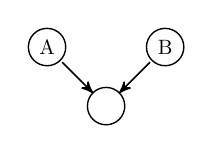
\begin{tikzpicture}[scale=0.75,transform shape]
		\tikzstyle{LabelStyle}=[fill=white,sloped]
		%  \tikzstyle{EdgeStyle}=[bend left]
		\Vertex[x=-1,y=0,LabelOut=false]{A}
		{
			\SetVertexNoLabel
			\Vertex[x=0,y=-1]{C}
		}
		\Vertex[x=1,y=0]{B}
		\tikzstyle{EdgeStyle}=[post]
		\Edge[](A)(C)
		\Edge[](B)(C)
		%  \Edge[label=$$](K)(F)
	\end{tikzpicture}
	\caption{\label{fig:marriage}Marriage}
\end{figure}

% Love is experience as the self of the ``married" identity in one's mind, while marriage is the construct in the world.

Now some cultures sustain polygamous marriages, and apparently these are functional enough to have persisted over the centuries. How can this be? We will discuss this in the section on \hyperref[sec:phirelhistra]{\textit{religious traditions}}.

\subsection{Nature of Anonymous Identity} \label{sec:natanoide}

When an anonymous act is performed within the mind of an identity $Q$, by definition it is an act for which no member will claim responsibility. Therefore it is unknown which of the known constituents of the mind was responsible for the act. But at the same time, clearly \textit{somebody in $Q$} did it. How can this be captured? Consider a simple $3$-member identity where an anonymous act $X$ has been performed (Fig.~\ref{fig:anonymous}). Identity $A$ knows it didn't perform the act and so models it as derivative of the compound of $B$ and $C$. Say $C$ didn't perform the act either, so $C$ models it as derivative of the compound of $A$ and $B$. $B$ actually performed the act, but since it is not accepting responsibility for it, $B$ must within the mind of $Q$ model the act as derivative of the compound of $A$ and $C$. None of the models agree, and they can argue till the end of the world who was responsible for what, but there's simply no way to know who is ``lying'' and who isn't. Instead, the only way the models can be consistent is if the act is agreed to have been performed by the intersection of the three models $\{A, B\} \cap \{B, C\} \cap \{A, C\}$, which is the empty set. Therefore, anonymous acts are those corresponding to the empty set $\varnothing$ of identities, which is in line with our axiomatic definition of anonymous identity in \autoref{def:idecon}. Note that this is the empty subset within the mind of $Q$, which can as such still be identified with ``some identity in $Q$.'' In this regard it is to be treated as different from the empty subset in the world external to $Q$. As such, while in set theory the empty set is unique, here an anonymous identity (as with all identities) is defined with respect to a particular identity context (although the anonymous identity of a mind does correspond to the representation of the world anonymous identity in the mind under a perception functor). To highlight this distinction, and as a matter of notation, given an identity $Q = (\mathcal{M}_Q, B_Q, \phi_Q)$ in a world $\mathcal{W}$, we will denote the anonymous identity of the world by $\varnothing_\mathcal{W}$ and the anonymous identity of the mind of $Q$ by $\varnothing_{\mathcal{M}_Q}$ or simply $\varnothing_Q$. Finally, note that in the above interaction, all of the individual identities are aware of the ``true'' model from their perspective, and this is the model that they will use \textit{internally} -- that is to say, in their own mind contexts.

\begin{figure}[htp]
	\centering
	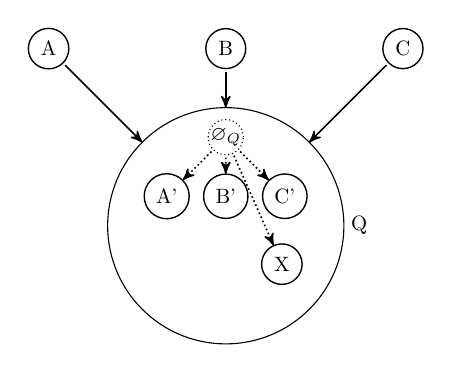
\begin{tikzpicture}[scale=0.75,transform shape]
		%\tikzstyle{LabelStyle}=[fill=white,sloped]
		%\draw[solid] (0,0) circle (2cm);
		\GraphInit[vstyle=Normal]
		\Vertex[x=-3,y=3]{A}
		\Vertex[x=0,y=3]{B}
		\Vertex[x=3,y=3]{C}
		{
			\tikzset{VertexStyle/.style = {draw=black,shape=circle,minimum size=4cm,inner sep=0pt}}
			\Vertex[x=0,y=0,LabelOut=true]{Q}
		}
		%\tikzset{VertexStyle/.append style = {draw=darkgray,text=darkgray}}
		{
			\tikzset{VertexStyle/.style = {draw=black,shape=circle,style=densely dotted,minimum size=0cm,inner sep=0pt}}
			\Vertex[x=0,y=1.5,L=$\varnothing_Q$]{QQ}
		}
		\Vertex[x=-1,y=0.5,L=A']{A1}
		\Vertex[x=0,y=0.5,L=B']{B1}
		\Vertex[x=1,y=0.5,L=C']{C1}
		\Vertex[x=0.95,y=-0.65]{X}
		\tikzstyle{EdgeStyle}=[post]
		\Edge[](A)(Q)
		\Edge[](B)(Q)
		\Edge[](C)(Q)
		{
			\tikzstyle{EdgeStyle}=[post,densely dotted]
			\Edge[](QQ)(A1)
			\Edge[](QQ)(B1)
			\Edge[](QQ)(C1)
			\Edge[](QQ)(X)
		}
		%\tikzset{EdgeStyle/.append style = {draw=darkgray,text=darkgray}}
	\end{tikzpicture}
	\caption{\label{fig:anonymous}Anonymous Identity}
\end{figure}

Now, in any context if we follow the known identity tree upward, we will eventually reach a set of identities for which there is no information about their genesis. These identities, following the same reasoning as in the previous paragraph, must also be modeled as anonymous, i.e. descended directly from the unique anonymous identity of the context. By considering the outermost world perceivable, we are led to conclude that all identities must ultimately derive from the anonymous identity of that world (reminiscent of the construction in set theory, via the cumulative hierarchy, of all sets in a Grothendieck universe by iterating set operations on the empty set), also depicted in Fig.~\ref{fig:anonymous}. Just as water takes the shape of any container, so does an anonymous identity take the forms of all identities. We will say more on the matter when we discuss below the ideas of ``energy'' and ``currency,'' which we consider as modeled by anonymous identity.

\section{Interpretation} \label{sec:interpretation}

As discussed earlier, identity can be seen as the substance of our reality. By its status in this regard, the models presented above allow us to reinterpret common ideas and institutions.

\subsection{Currency} \label{sec:currency}

% Amount of "value" in the identity as proportional to the amount of identities expressed, so entropy generates value
%TODO: consider mentioning how anonymous nature of currency itself provides anonymous exchange -- no one can institute a policy like "I won't accept X's money"

A single organism (such as a human) must feed itself, defend itself against predators and competition, and must have access to a safe location for resting. When such organisms band together into larger groups, economies of scale emerge enabling the division of responsibilities into focused functional groups, which allows the requirements of all members to be aggregated and handled in batches. The group can be said to comprise a higher organism, i.e. a hive identity. As the organism grows in scale, it becomes more challenging to properly assess its needs, and so a market economy emerges where these needs can be determined organically: a shortage of a particular resource drives up the incentive to address it within the organism, and when that incentive exceeds the opportunity cost for some subset of members to address it, that subset rises to the need.

Initially, the organism may sustain a barter economy, but over time, trade in specific goods and services becomes cumbersome and it becomes apparent that the objective of the implicit market economy is to accord -- \textit{within the mind context} -- a level of access to goods and services to a constituent that is commensurate with the value of the goods and services provided by it. It is soon realized that this may be more precisely captured in a form of monetary currency.

When the organism encounters other human settlements in the world, a form of currency exchange is developed that allows trade between them. We can say that the value possessed by a constituent represents a fraction of the total value in the \textit{mind}, which is convertible into a fraction of total value in the \textit{world}, and so on, in a self-similar manner. This fraction is naturally characterized as a real number between $0$ and $1$, which we can call the \textit{wealth} of a constituent within that context.

Observe further that under this characterization, the fraction of context value contained in a constituent $q_i$ can be interpreted as the proportion of the ``amount'' of identity of $Q$ that is contained in $q_{i}$, since $q_{i}$ ``controls'' the functioning of $Q$ in the world precisely to the extent of its own wealth within the mind $\mathcal{M}$ of $Q$. And in the same manner, $Q$ guides the functioning of the world identity to an extent commensurate with its wealth in the context $\mathcal{W}$, and so on. In this sense, since all constituents in a context derive from the anonymous identity of that context, we can equate the totality of wealth in a mind with the anonymous identity of the mind (i.e. $1.0 \varnothing_Q$), which in turn we may as well equate with the identity itself as it exists in the world (i.e. $1.0 \varnothing_Q = w_{\mathcal{W}}(Q) \varnothing_{\mathcal{W}}$).

\begin{defn}[Wealth]
	In any context $\mathcal{W}$, \emph{wealth} is a function defined on $\mathcal{W}$ that maps each constituent $q \in \mathcal{W}$ to a real number $w_{\mathcal{W}}(q) \in [0, 1]$ at a particular point in time, and is recursively determined as:
	\begin{equation} \label{eq:wealth}
		\begin{split}
			w_{\mathcal{W}}(\varnothing_{\mathcal{W}}) &= 1.0 \\
			w_{\mathcal{W}}(q) &= \sum_{i} w_{Q_i}(q) \cdot w_{\mathcal{W}}(Q_i) ;
		\end{split}
	\end{equation}

	where the $Q_{i}$ correspond to minds in $\mathcal{W}$ to which $q$ belongs, and $w_{x}$ represents wealth in context $x$.
\end{defn}

Therefore, currency can be seen as a manifestation within the systems of human society of anonymous identity. This can be empathized with when one considers that every dollar (or whatever unit of currency) is equivalent to every other dollar and devoid of identity without reference to its context (would you accept a form of currency without knowing which country it's from?), and in sufficient quantities can ``take the form'' of any identity in the context in a process we call ``purchasing.'' Money can enable any individual or enterprise, regardless of form or purpose, and so it too is ``like water.''

Now with money established as corresponding to ``quantity'' of anonymous identity, we observe further that maintaining discrete quantities of currency within constituents for any nonzero extent of time is inefficient. Learned wisdom has it that one must keep money ``moving,'' but this notion isn't captured formally within our economic systems. It could be useful if such a continuous, time-variant system of currency were adopted, where all transactions occur as rates and times and not necessarily as discrete quantities. We could call such a quantity the \textit{influence} of an identity in a context.

\begin{defn}[Influence]
	For identities $q, r \in \mathcal{W}$, an \emph{influence} applied by $q$ on $r$ is a function $n(t)$ such that:
	\begin{equation}
		\begin{split}
			\Delta w(r) &= \! \int_{0}^{T} n(t)\,dt \label{eq:influence}, \text{ and} \\
			\Delta w(q) &= - \Delta w(r) ;
		\end{split}
	\end{equation}

	where $n$ is the influence applied on $r$ by $q$, $\Delta w$ is the change in wealth of an identity, and $T$ is the duration for which the influence is applied. An edge in a bodhitree can be interpreted to entail such an influence.

\end{defn}

Note that a one-time discrete exchange of money would be a special case of the above, and can be captured by employing an impulse function as the influence. In general the influences into and out of an identity should be at a steady state, i.e. their sum should equal zero:

\begin{equation}
	\sum_{i} n_i(t) = 0 .
\end{equation}

Influence and wealth are developed further in the section below on \hyperref[sec:ecogovintpro]{Economies}.

\subsection{Identity and the Brain} \label{sec:idebra}

The natural application of the identity model is, of course, to the brain. Before we continue, it is worthwhile to reaffirm that our experience of the physical world exists entirely within a mental representation of that world which, we proffer, is in terms of identities. Within this representation, actions that we take actually manifest in the physical world, and interactions that occur in the physical world occur also in this representation. In other words this representation in the mind is in a state of persistent equivalence with the physical world, which we identified earlier as a form of categorical equivalence or adjunction. We will generally avoid speaking directly of this equivalence between actions in the mind and actions in the physical world, and will make no distinction between them. Its existence, however, has important implications which we address in the section on \hyperref[sec:natphe]{natural phenomena}.

\subsubsection{The Self} \label{sec:theself}

Anything we can conceive of as a thing is an identity in the sense of this document. Clearly a person meets this requirement and is an identity. Following from the definition of identity, the person defines a mind context relative to the world, which can be seen to correspond to the traditional idea of a mind (of course the terminology was chosen for this reason). By \autoref{lem:maya}, all things in the world have a representation in the mind as thoughts (a claim supported by our ability to think about objects even when we close our eyes). Now as a person, one is able to conceive of oneself, and is able to act as a causative agent in the form of this ``self.'' The conception of the self can be seen to derive also from \autoref{lem:maya}: since every thing is represented in the mind as a thought, the identity itself, being a thing in the world, must exist in the mind as a thought, or a representation of itself. This natural characterization is shown in Fig.~\ref{fig:self}, and corresponds to the notion of the ``self.''

\begin{figure}[htp]
	\centering
	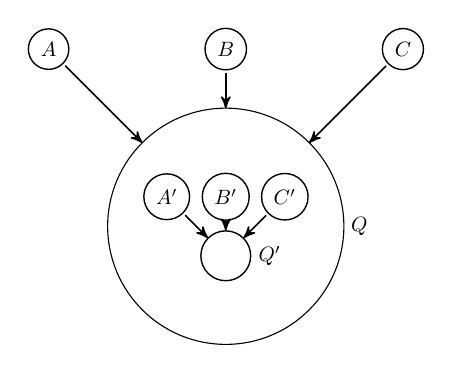
\begin{tikzpicture}[scale=0.75,transform shape]
		%\tikzstyle{LabelStyle}=[fill=white,sloped]
		%\draw[solid] (0,0) circle (2cm);
		\GraphInit[vstyle=Normal]
		\Vertex[x=-3,y=3,L=$A$]{A}
		\Vertex[x=0,y=3,L=$B$]{B}
		\Vertex[x=3,y=3,L=$C$]{C}
		{
			\tikzset{VertexStyle/.style = {draw=black,shape=circle,minimum size=4cm,inner sep=0pt}}
			%\SetVertexNoLabel
			\Vertex[x=0,y=0,L=$Q$,LabelOut=true]{Q}
		}
		%\tikzset{VertexStyle/.append style = {draw=darkgray,text=darkgray}}
		\Vertex[x=-1,y=0.5,L=$A'$]{A'}
		\Vertex[x=0,y=0.5,L=$B'$]{B'}
		\Vertex[x=1,y=0.5,L=$C'$]{C'}
		{
			\tikzset{VertexStyle/.append style = {shape=circle,minimum size=24pt,inner sep=0pt}}
			%\SetVertexNoLabel
			\Vertex[x=0,y=-0.5,L=$Q'$,LabelOut=true]{Q'}
		}
		\tikzstyle{EdgeStyle}=[post]
		\Edge[](A)(Q)
		\Edge[](B)(Q)
		\Edge[](C)(Q)
		%\tikzset{EdgeStyle/.append style = {draw=darkgray,text=darkgray}}
		\Edge[](A')(Q')
		\Edge[](B')(Q')
		\Edge[](C')(Q')
	\end{tikzpicture}
	\caption{\label{fig:self}The Self}
\end{figure}

\begin{defn}[Self]
	Given an identity $Q = (\mathcal{M}, B, \phi, \mu, \omega)$ in a world $(\mathcal{W}, \psi)$, the \emph{self} of $Q$ is defined to be the thought $Q' = (\mathcal{M}', B', \phi', \mu', \omega')$ within $\mathcal{M}$ such that $Q' = \mu(Q)$.
\end{defn}
% Is the axiom of universes satisfied (and obviated) by the self?

Note that as all identities are qualitatively equivalent, in particular $Q'$ is as fully an identity as $Q$, and can sustain a representation of itself within it. Similarly, the identities $A'$, $B'$, and $C'$ are representations of $A$, $B$ and $C$ within $Q$, and can harbor representations of each other within themselves within $Q$, and so on. Furthermore, each constituent in the mind of $Q$ can represent also the self of $Q$, i.e. can conceive of $Q'$ -- this fractal nature can be experienced when we think about doing something, for example, and then think about thinking about doing that thing (in Fig.~\ref{fig:self}, this would be experienced as the self of the thought (e.g. $A'$) that is thinking about the action of the self (i.e. $Q'$) of $Q$). This is exactly the kind of self-recursive nature described by Hofstadter\cite{geb}, corresponding approximately to what he refers to as a ``strange loop.''

Further, it appears that when we think of anything, we ``are'' the self of that thought. Thinking of a book in one's field of view is experience as the self of that book-as-a-thought. Thinking of the self, we are the self of the self.
%Following this will no doubt yield some fascinating insights into the nature of nirvana. I seem to recall Shankara concluded that this strange loop nature implied that atman=brahman since there is always an "observer"

\subsubsection{Language} \label{sec:language}

Linguistic communication structurally can be seen as an instance of a more general process of conveyance of identity trees from one mind to another via interaction. As such, spoken language (for example) can be characterized as an action of the identities in the mind on identities in the world (which includes our physical forms and in particular our vocal cords), followed by, from the perspective of the other person, an action of the world (including their physical forms and in particular their auditory structures) on the identities in their mind. This would be facilitated at either end by an expression and a perception functor, respectively. Under this description, the ``deep structure'' described by Chomsky\cite{chomsky} would correspond to the identity architecture of the mind, some subset of which is isomorphic to the linguistic expression. This entire preceding interaction would be represented in the minds of the participants as existing within a nested mind constituted by (representations of) the two participants in the conversation. In the mind of one of the participants, this identity would communicate ``linguistically'' with other identities in his mind, ``spreading the word,'' as it were. Over time, the information gleaned in the conversation would be incorporated into the identity structure of the mind as a whole, with any remaining particulars being recalled from this identity as needed. This ``social'' nature of the identities in the mind is reminiscent of Minsky's ``society of mind,''\cite{minsky} where he considers specialized ``agents'' in the mind that work together in hierarchies to accomplish complex tasks.

%Language has monoid structure...

Language itself can be seen to consist primarily of words (or more precisely \textit{lexemes} -- fundamental semantic units of which words are considered to be specific forms). Words are identities that exist in a persistent and universal lexicon, and correspond to models that are relevant in our experience of the physical world. Identities corresponding to words are to be considered isomorphic across minds (although in practice they may not be so, we reinforce this isomorphism by having universally-agreed-upon resources for arbitration of any disagreements, in the form of dictionaries and encyclopedias\footnote{which reinforce isomorphism by the transitivity of the relation of being isomorphic.}).

Language obviously consists of more than words, however. Sentences represent ordered subsets of words which serve to construct and communicate identities that are not part of the standard lexicon (or else we would just use the word corresponding to the intended communication). The reason we resort to sentences instead of simply extending our lexicon to contain any novel identities is that if indeed ``subsets of words'' are what it takes to capture our experience, then representing new ideas directly as identities would require that each person carry around a representation of $2^{Card(W)}$\footnote{In fact, as mentioned previously, sentences are \textit{ordered} subsets and not just subsets. But since the order can be varied under alternate grammatical constructions (e.g. ``The girl threw the ball'' vs. ``The ball was thrown by the girl''), we consider the weaker model of unordered subsets of words as it is sufficient to express the argument. The number of (unordered) subsets of a set of size $n$ is $2^{n}$, which is strictly greater than $n, \forall n$.} words in their minds, where $W$ is the set of words they would have to know if they used sentences instead. This also implies that with a countably infinite number of words, we can represent an uncountable number of ideas using sentences, and therefore it is a superior computational model regardless of any efficiency considerations of storing additional words in one's head.

As such, sentences represent computations that construct new identities from available ones. As an example, we can envision in a typical sentence each word and in particular the nouns as corresponding to identities in the lexicon; adjectives as conveying heredity of an identity that is not part of the lexicon -- and therefore enabling the recipient to construct this identity in their mind; verbs as conveying actions of identities on other identities and therefore communicating the genesis of new identities, which is simulated in the mind of the listener.

\subsubsection{Cognition} \label{sec:cognition}
% The basic task can be characterized as: given an action of an identity, determine its body. the most general identity of which the image is a quotient subidentity - likely related to some kind of universal construction
% applying functors until an identity becomes anonymous in some context yields its properties as the body of that identity
% the body appears to be the relevant set to calculate information on

When an experience in the physical world $\mathcal{W}$ is apprehended by a person $p = (\mathcal{M}_{p}, \phi) \in \mathcal{W}$, it can be seen to be an action of identities in the representation (via the perception functor) of the world in the mind, on the self. This action translates in the mind of the self into actions on the identities -- that is, the thoughts -- of the self. This further translates into actions on the selves of the thoughts of the self, and so on (since we embody a particular (single) self at any point in time, it's likely that each computation is undertaken only when we embody a self affected by that action. This could represent the nature of the interactions that are described below in \hyperref[sec:dreams]{Dreams}). Each action gives rise to a reaction and to genesis, and these are all aggregated outward to form the reaction of the self in the mind, which, via the expression functor, translates into the reaction of the person to the experience in the physical world. The nature of this aggregation could be modeled as corresponding to the extent that the identity of $p$ (in the sense of anonymous identity, i.e. ``quantity'' or wealth) is expressed in her constituent thoughts. All thoughts in the self, and thoughts within the minds within the self, weigh in on each issue in terms of their reactions to it, and are considered to the extent of their influence in the relevant contexts. This is discussed further in the section on \hyperref[sec:ecogovintpro]{Economies and Government}.

Beyond representation of the physical architecture of the world, our minds also represent identities such as human motivations and communications that are present in minds within the physical world (note that communications exist not within a human mind but in the mind of the hive identity constituted by participants in the communication. These participants form the body of this hive identity) that do not themselves have a faithful or persistent physical representation. We can understand this representation as existing in minds within our mind that are representations of those minds in the physical world. That we are able to construct these representations derives from the partial order defined by bodhitree evolution; that is, since new identities in a context manifest via actions of existing identities in the context, evolution of a context cannot simply occur arbitrarily within all possibilities supported in the universe. When an identity in the world is considered, therefore, we are able to inductively determine a heredity based on other known and inferred identities in the world and in minds within the world. In particular, every identity in the world has a defined heredity in the mind, even if this is simply that that identity is anonymous (i.e. descended directly from the unique anonymous identity of the world). This heredity construction of a given identity can be seen to correspond to our faculties of reasoning and cognition.
% clarify relationship to Kant's "thing-in-itself" and "noumena"

Edges in a bodhitree as discussed earlier can be interpreted as entailing influence, and as such, heredity construction could include assignment of likely influence of each inferred ancestor. Since influence is in terms of fractions of a particular anonymous identity and therefore takes values between $0$ and $1$, this could naturally correspond to an interpretation as probabilities, and it's possible a Bayesian or other probabilistic model could inform this process of heredity construction. In general in probability theory, the likely occurrence of any event has an associated distribution, which itself has an associated ``confidence'' distribution, which in its turn can also have a confidence distribution, and so on. These nested confidence distributions appear to correspond to models as nested selves.

\subsubsection{Consciousness and Memory} \label{sec:conmem}

By the definition of identity, the mind is a persistent representation of the world and every thing in the world is present in the mind to the extent that it is apprehended. Now we examine \autoref{lem:maya} to derive yet another noteworthy implication. Since representations of things exist in minds but thoughts don't exist in worlds, the lemma also implies that any identity $q$ within a world $\mathcal{W}$ contains a full internal representation of every mind to which it belongs\footnote{The mind of $q$ could be considered as the context to which all ``classes'' in each mind of which $q$ is a member belong, serving as a containing context for any identity that could be conceived from the constituents of those minds. This would obviate the need for an axiom of universes.}. That is, if $q$ constitutes $n$ things in $\mathcal{W}$, then each of those $n$ minds are represented in $q$, although of course no representation of those minds necessarily exists in $\mathcal{W}$. As an illustration, in Fig.~\ref{fig:awareness}, the entire figure is also present within $B$. Taken together with the ``strange loop'' fractal pattern of self manifestation discussed in \autoref{sec:theself} above, this aspect is highly reminiscent of the Buddhists' doctrine of ``interpenetration'' of all reality, as embodied in their vivid account of ``Indra's Net.''\cite{avatamsaka}

This representation in $B$ does not, however, include any identities within the minds of $A$ or $C$ that are not present in the worlds $P$ and $Q$. This persistent internal representation of myriad worlds, together with the recursive representation of the self described previously, likely constitute our experience of ``consciousness''; and memory, specifically the process of ``recollecting'' something can be seen to be the act of utilizing available information to assemble the heredity of the mind within which the desired information exists, and then simply deriving a world-representation (via successive expression functors) of the identity corresponding to the memory. This world-representation would include any modifications or retractions imposed by the contexts along the path to the world.

\begin{figure}[htp]
	\centering
	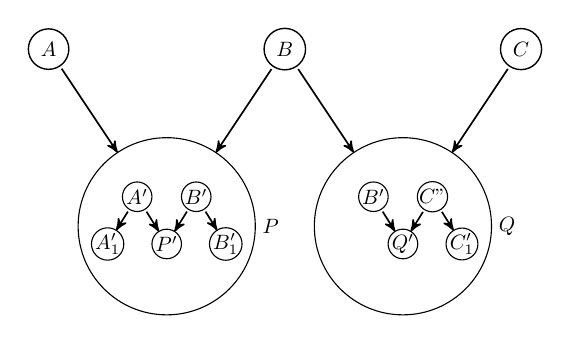
\begin{tikzpicture}[scale=0.75,transform shape]
		%\tikzstyle{LabelStyle}=[fill=white,sloped]
		%\draw[solid] (0,0) circle (2cm);
		\GraphInit[vstyle=Normal]
		\Vertex[x=-4,y=3,L=$A$]{A}
		\Vertex[x=0,y=3,L=$B$]{B}
		\Vertex[x=4,y=3,L=$C$]{C}
		{
			\tikzset{VertexStyle/.style = {draw=black,shape=circle,minimum size=3cm,inner sep=0pt}}
			%\SetVertexNoLabel
			\Vertex[x=-2,y=0,L=$P$,LabelOut=true]{P}
			\Vertex[x=2,y=0,L=$Q$,LabelOut=true]{Q}
		}
		{
			\tikzset{VertexStyle/.style = {draw=black,shape=circle,minimum size=0.5cm,inner sep=0pt}}
			%\SetVertexNoLabel
			\Vertex[x=-2.5,y=0.5,L=$A'$]{A'}
			\Vertex[x=-1.5,y=0.5,L=$B'$]{B'}
			\Vertex[x=-2,y=-0.3,L=$P'$]{P'}
			\Vertex[x=-3,y=-0.3,L=$A_{1}'$]{A"}
			\Vertex[x=-1,y=-0.3,L=$B_{1}'$]{B"}
			\Vertex[x=2.5,y=0.5,L=$C"$]{C'}
			\Vertex[x=1.5,y=0.5,L=$B'$]{B`}
			\Vertex[x=2,y=-0.3,L=$Q'$]{Q"}
			\Vertex[x=3,y=-0.3,L=$C_{1}'$]{C"}
		}
		%\tikzset{VertexStyle/.append style = {draw=darkgray,text=darkgray}}
%		{
%			\tikzset{VertexStyle/.append style = {shape=circle,minimum size=24pt,inner sep=0pt}}
%			%\SetVertexNoLabel
%			\Vertex[x=0,y=-0.5,L=$Q'$,LabelOut=true]{Q'}
%		}
		\tikzstyle{EdgeStyle}=[post]
		\Edge[](A)(P)
		\Edge[](B)(P)
		\Edge[](B)(Q)
		\Edge[](C)(Q)
		%\tikzset{EdgeStyle/.append style = {draw=darkgray,text=darkgray}}
		\Edge[](A')(P')
		\Edge[](B')(P')
		\Edge[](A')(A")
		\Edge[](B')(B")
		\Edge[](B`)(Q")
		\Edge[](C')(Q")
		\Edge[](C')(C")
	\end{tikzpicture}
	\caption{\label{fig:awareness}``Awareness''}
\end{figure}

\subsubsection{Dreams} \label{sec:dreams}

Every night of every day, every person in the world sleeps. And dreams. We've been doing this for thousands, millions of years. But the explanation of the nature of dreams has largely eluded us. Sometimes we wake from one and the recollection of it quickly escapes description. The dream is on the tip of one's tongue, and yet hopelessly out of reach. We've all experienced this; why does it happen? We attempt explanations in terms of identities.

When we sleep, we cease taking sensory input from the physical world, and the mind context corresponding to activity in the physical world -- including the self in that context -- ceases to be expressed. But as the world fades from experience the identities in the mind remain, and continue to interact as they always do. In the absence of the physical world and ``the'' self, we experience these interactions in the mind as the selves of the participating thoughts. Many of these thoughts may be sophisticated aspects of our full selves, and so these dreams we can remember more easily, since they are closer to our experience.

But so many other dreams make so much sense to us as we sleep, and then suddenly at the instant of waking they seem to confound description. This phenomenon could be because the thoughts that experience them are more primitive aspects of ourselves, and the worlds they inhabit may be quite different from the physical world. Therefore, the models (i.e. identity trees) used by them to describe their experience may be alien to experience in the physical world, and these models would be unlikely to correspond fully to words we use. For example, words like ``mother,'' ``neighbor,'' ``sky,'' or ``tree'' correspond to identities in the physical world. But in the minds within the mind, subsets of trees corresponding to these words may be employed to capture experiences relevant in those worlds, which would only be primordial aspects of physical world-concepts. So some aspect of ``neighbor'' may in a thought be used to describe an experience, but when we wake into the physical world, ``neighbor'' no longer captures that concept and we find our language inadequate to describe the notion. Such a dream quickly fades from expressibility. The same reasoning could also explain why memories from early childhood and infancy cannot be recollected, even by young children. Those experiences do not correspond to models (and words) used later in life.

\subsubsection{Music} \label{sec:music}

In music, tones of frequencies that are power-of-2 multiples apart have the same periodic structure and so sound the same to us, except ``higher'' or ``lower.'' This can be modeled as equivalence classes of pitches under the relation of ``sounding the same,'' and the classes under this conception then represent musical notes\footnote{In musical set theory such classes are called ``pitch classes'' but, unless we are mistaken, it seems that such a pitch class is just a formal model for the more informal idea of a note, and so we do not make this distinction for the moment and opt for the more familiar terminology.}. We can conceive musical notes to be identities. It follows that a collection of notes defines a hive identity (a ``chord'') and an identity context. Such a characterization is already extant in musical set theory\cite{musicalsettheory}, where such a context is called a musical set, or pitch-class set. The identity picture could be seen to provide a cognitive basis for studying music via musical set theory. It also motivates some generalizations which could conceivably inform further development.

A musical context can express relationships between the constituent notes in the form of hive identities constituted by them. It is often desirable to have a preferred note -- called the \textit{tonic} -- such that all other notes in a context are considered in terms of their relationship to this note. Such a construction could be captured as shown in Fig.~\ref{fig:key}, and corresponds to the notion of a musical key. We observe that, for example, the keys of \textit{C major} and \textit{A minor} are differentiated only by choice of tonic, which is captured by this construction. We can in general always construct a ``chromatic'' context composed of all available notes, for example all $12$ notes in the standard 12TET. Under our definition of a key, we can then define ``chromatic keys'' on this chromatic context by selecting a particular note as tonic. Note that members of a key are not notes but relationships; in the key of \textit{F major}, the identity of the note \textit{A} is ``a third.'' The ``underlying note'' \textit{A} is easily obtained by applying an expression functor, treating the relevant chromatic context as the world. Similarly we can consider this chromatic context to exist as a mind in the world of frequencies of sound, and then applying an expression functor to the note provides us with the underlying frequency, in this case $440$ Hz.

\begin{figure}[htp]
	\centering
	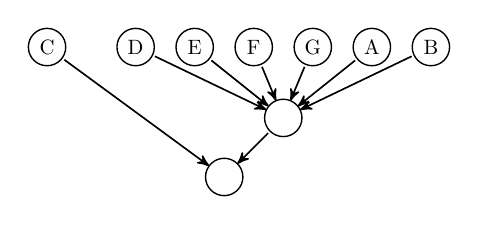
\begin{tikzpicture}[scale=0.75,transform shape]
		\tikzstyle{LabelStyle}=[fill=white,sloped]
		%  \tikzstyle{EdgeStyle}=[bend left]
		\Vertex[x=-2,y=0]{C}
		\Vertex[x=-0.5,y=0]{D}
		\Vertex[x=0.5,y=0]{E}
		\Vertex[x=1.5,y=0]{F}
		\Vertex[x=2.5,y=0]{G}
		\Vertex[x=3.5,y=0]{A}
		\Vertex[x=4.5,y=0]{B}
		{
			\SetVertexNoLabel
			\Vertex[x=2,y=-1.2]{H}
			%\SetUpVertex[FillColor=gray!70]
			\Vertex[x=1,y=-2.2]{J}
		}
		\tikzstyle{EdgeStyle}=[post]
		\Edge[](D)(H)
		\Edge[](E)(H)
		\Edge[](F)(H)
		\Edge[](G)(H)
		\Edge[](A)(H)
		\Edge[](B)(H)
		\Edge[](H)(J)
		\Edge[](C)(J)
		%  \Edge[label=$$](K)(F)
	\end{tikzpicture}
	\caption{\label{fig:key}Musical Key}
\end{figure}

One usually says that compositions are in a particular key, for example, ``Waltz in C-sharp minor.'' We can consider it equivalent to say that musical compositions are in a particular identity context. As such, some natural generalizations that could be explored include keys other than major and minor (such as the chromatic keys already discussed), and musical contexts composed of multiple keys (such contexts are no doubt already in use). Such a characterization could enable the study of the existing rules of music in a generalized form that could be applied in other non-standard tunings such as 19TET or forms of just temperament (musical set theory seems to be already applied in this manner). Additionally, by treating a chromatic key as a world and more specific keys (e.g. \emph{C major}) as minds within that world, it seems to be the case that musical transformations such as transpositions and modulations can be achieved by successive application of expression and perception functors.

Similarly, rhythm can also be interpreted in terms of identities. For example, the standard interpretation of the $\frac{6}{4}$ time signature ($6$-count) as distinct from the $\frac{3}{4}$ signature ($3$-count) -- that the emphasis on the first three beats is different from the second three beats -- appears to correspond to a characterization as a hive identity derived from $3$-count and $2$-count, and having aspects of both. Lewin in \cite{gmit} studies both musical notes and rhythms in terms of an abstract group-based structure he calls a Generalized Interval System (GIS). This unity in the mathematical structures of melody and rhythm seems to further ground the case for the applicability of identities to rhythm as well.

Finally, musical compositions are constructs that usually possess some high-level defining structure: a song may be composed of recurring sections such as a verse and chorus. Within each of these sections are distinct phrases consisting of particular melodies along with the accompanying harmonies, each of which of course consists of notes (generally) in the given key. At the highest level this entire structure may comprise a single movement, of which the composition may have several (in classical music, for example). And at the lowest levels, melodies and rhythms may possess further ornamentation -- melodies within melodies, and rhythms within rhythms, as especially evident in the Carnatic and Hindustani classical traditions. In all cases, the nested patterns must ``fit'' into the higher patterns if the identity of the higher pattern is to be expressed. As such, at a high enough level, there must exist a single meter into which all the patterns fit, which unifies and reinforces its identity as a single composition, as opposed to being just an overlapping multitude of musical patterns. This is indeed usually the case. This ``fractal'' structure in music betrays its ties to identities, and suggests that each level described may be studied independently in terms of identities. In music theory, Schenkerian analysis\cite{schenker} studies this type of nested structure.

There have been several other mathematical examinations of music and musical elements, for e.g. \cite{musicmath} and \cite{musselfsim}. As music is a cognitive phenomenon, we believe it must be the case that identity representation provides the basis for this mathematical structure.

\subsubsection{The Sense of Smell} \label{sec:sensme}

Similar identity abstractions can be found in our experience of the sense of smell. Different foods, for example, have different smells that we can pick out. Garlic smells a certain way, and onion another. Fish has a particular smell, as does sesame oil, truffle oil, mustard, chicken, steak, rice. But when we smell our favorite food -- eggplant curry, say -- as we are about to eat it, we don't smell the onion and the garlic and the eggplant. We smell \textit{eggplant curry}. Certainly, we could pick out the garlic within that smell just as we can pick out individual musical notes in a chord if we try. But our olfactory experience of the eggplant curry is a distinct one in its own right. Additionally, things could smell ``like Chinese food'' which obviously corresponds to a hive identity rather than a particular Chinese dish. The formulation of perfumes follows a similar identity construction -- different molecules possessing desirable smells are combined to create a unique olfactory experience deriving from the properties of each of those molecules\cite{smellmolecules}.

\subsubsection{The Sense of Taste} \label{sec:sentas}

Food preparation is the practice of taking a number of ingredients and preparing them, putting them together in certain ways to create something that is more than the sum of its parts. If eggplant curry simply tasted like eggplant and like garlic and like onions, then one may as well eat each of those things separately, in any order. But our experience of the eggplant curry is quite different, and rather more enjoyable, than of any of its ingredients. Each dish is experienced as a hive identity comprised by its ingredients. Just as in music, where two notes may sound dissonant when played together, but consonant when played as part of a more complex chord, so it is with food where ingredients that taste bad together by themselves (e.g. wasabi and soy sauce) can taste good when part of a more complex preparation (sushi).

\subsubsection{The Sense of Sight} \label{sec:sensig}

Our perception of color exhibits identity structure. Red and blue combined is purple -- a new color with a unique experience, distinct from either of its constituents. In other words, colors when combined yield other colors -- an obvious but noteworthy state of affairs. Our visual perception of objects can also be seen as exhibiting identity structure. Visual perception is entirely in terms of colors, contrasts, intensities in a two-dimensional matrix. But we don't see just colors and contrasts, we see \textit{things} -- books, laptops, people, cats. Each of these objects in our visual experience corresponds to a hive identity possessing various characteristic features which are themselves composed of characteristic features, and so on. A person could be characterized as having black hair (a purely visual characterization, irrelevant outside of visual perception), wearing a t-shirt. Black hair itself would have attendant features such as textures and reflectivity and spatial relationship with other identities such as face and body. In the field of computer vision, probabilistic models are developed to identify objects in scenes. Such models could benefit from a basis in identity architecture, and also be generalized to represent all of perception and reasoning, since after all, all forms of perceptual representation and reasoning are (we believe) in the same terms -- that of identities. This envisioning is consistent with proposals by Mountcastle\cite{mountcastle} and by Hawkins\cite{hawkins}.

\subsubsection{The Sense of Touch} \label{sec:sentou}

If we close our eyes and run our hands over an unknown object in our vicinity, we naturally develop a characterization such as ``a small box with a smooth top and a coarse bottom, with a metallic latch.'' When we compare this to the actual sensory input which could be expressed as something like ``edge, corner, edge, corner, smooth, edge, corner, rough, edge, cold,'' it's easy to see that the sense of touch also is in the hierarchical terms of identity. In the sense of kinesthetics, identities manifest in our execution of complex physical maneuvers such as playing sports, engaging in martial arts, dancing, acrobatics. These could all be seen as corresponding to hive identities composed of all the attendant minute motions. When we pick up a pen that has fallen to the ground, we don't imagine moving our hands and fingers together with our arms and waists and knees and straightening out by shifting our weight a certain way and then placing the pen back on the table in another subtle and clever hand-and-arm gesture. We simply think of picking up the pen and putting it back on the table -- a hive identity we constitute by all those minutiae. Indeed, this can be seen as an i-morphism from this identity structure in the mind to the set of endomorphisms of the relevant identity structures in the world (including even our own physical form), i.e. an identity action as described in \autoref{sec:matmod}.

% Locomotion in the physical world forms a group. Why is this apt? Well for one thing, it means being able to undo any treacherous motion, e.g. pull one's hand back out of a thorny bush, walk backwards from a precipice, etc.

\subsection{Privacy} \label{sec:privacy}

Identities motivate a natural model for privacy; indeed, privacy itself may be seen as derivative of intrinsic notions of identity. Actions of an identity (in both the literal and algebraic sense) on other constituents in a context give rise to genesis of new identities, and we consider this to fully characterize how information is manifested in a context.

In natural phenomena, identity contexts emerge implicitly (i.e. via genesis; also see \autoref{sec:natphe}), while in human societies, contexts emerge implicitly but can also be conceived of in a persistent way, and actions can be taken in accordance with these perceived identity contexts (which we referred to as ``absolute'' contexts earlier). For example, if a citizen of a small town were to stand in the town square and make a proclamation, citizens of the town who are witness to it feel free to discuss it with other townsfolk who were not present there. They understand that proclamation to have occurred in the mind of the town as a whole. In comparison, if one individual were to make a private disclosure to another (``I'm Batman.''), the latter would generally feel impelled to share that disclosure with no one else; that is, both individuals represent this disclosure to have occurred in the mind constituted by just those two individuals. It's a ``secret.'' We observe in passing that secrets as identity contexts can have (as is familiar) any number of participants (constituents) (``I'm only telling you guys -- don't tell anyone else''), but due to anonymous effects (\autoref{sec:anoide}), a secret is only enforceable in the physical world if it is shared between a maximum of two individuals.

\begin{figure}[htp]
	\centering
	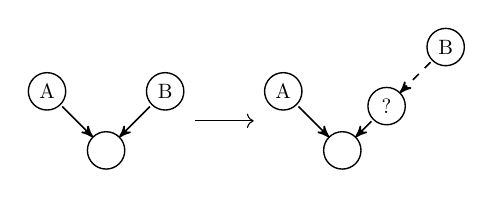
\begin{tikzpicture}[scale=0.75,transform shape]
		\tikzstyle{LabelStyle}=[fill=white,sloped]
		%  \tikzstyle{EdgeStyle}=[bend left]
		\Vertex[x=-3,y=0,LabelOut=false]{A}
		{
			\SetVertexNoLabel
			\Vertex[x=-2,y=-1]{C}
		}
		\Vertex[x=-1,y=0]{B}
		\tikzstyle{EdgeStyle}=[post]
		\Edge[](A)(C)
		\tikzstyle{EdgeStyle}=[post]
		\Edge[](B)(C)
		\draw [->] (-0.5,-0.5) -- (0.5,-0.5);
		\Vertex[x=1,y=0,LabelOut=false,L=A]{A'}
		{
			\SetVertexNoLabel
			\Vertex[x=2,y=-1]{C'}
		}
		\Vertex[x=3.75,y=0.75,L=B]{B'}
		\Vertex[x=2.75,y=-0.25,L=?]{D}
		\tikzstyle{EdgeStyle}=[post]
		\Edge[](A')(C')
		\Edge[](D)(C')
		\tikzstyle{EdgeStyle}=[post,dashed]
		\Edge[](B')(D)
		%  \Edge[label=$$](K)(F)
	\end{tikzpicture}
	\caption{\label{fig:privacy}Privacy: Association}
\end{figure}

We propose the following properties for the evolution of persistent identity contexts:

\begin{enumerate}

\item Within a context, an identity may declare or revoke an association to a child identity at any time. This results in a new child context with the modified tree. (\emph{association})

\item Any thought can act as the self. (\emph{presentation})
%TODO: this isn't the whole story. earlier math seems to indicate only actions of the self are actions in the world and not those of other constituents. but how does the self act at all? work out math for this -- I think monads are what are needed. and/or could be a currency-based construction in the self that, once all inputs are added and aggregated to a "maximal structure" in terms of these inputs, occurs. fourier transform could also be related -- once all the inputs are added to extents (magnitudes) corresponding to energy/currency, the result is the fourier sum "waveform" -- the combined identity/action.
	\begin{enumerate}
		\item An identity can act as any of its descendants (but descendants cannot act as ancestors).
		\item An identity can act as a ``dissociated identity.'' Acting as a dissociated identity is equivalent to acting anonymously in the world, but with the ability to ``reclaim'' the action being preserved.
	\end{enumerate}

\item World-representations of any thoughts that are not descendant from the self (and which are not mind-representations of things) should be trivial. In other words, identity trees within a mind should not in general be accessible from the world. (\emph{privacy})

\item It should be impossible (``hard'') to identify as descendant from a non-ancestor identity. (\emph{authentication})

\item It should be impossible (``hard'') to assert the association of an identity with one of its ancestors or descendants if that association has not been declared. (\emph{confidentiality})

\end{enumerate}

The first three properties are the core aspects, capturing and generalizing our everyday intuitions about privacy in human interactions. The first two enable Bruce Wayne and Batman to be two separate people to the world, and the same person to a few trusted aides. These can also be thought of as enabling an identity to act via a distinct ``identity proxy'' for each action it takes in the world, and further enabling the ability to associate or dissociate these proxies (and the associated actions) at any time. This type of pruning of one's identity tree could be seen as an explicit construction of one's so-called ``narrative identity''\cite{narrativeidentity} and is stronger than what we are practically able to achieve in human interactions in the physical world. The third property ensures our intuition that information in a particular context is not accessible to outsiders. This and the last two properties ensure integrity of the identity architecture and may be accomplished cryptographically. For this purpose, schemes based on Identity-Based Encryption (IBE) as proposed by Shamir\cite{shamir} and developed by Boneh and Franklin\cite{boneh} and by Cocks\cite{cocks} may be applicable.

Within a particular world $\mathcal{W}$, as already discussed, the anonymous identity $\varnothing_\mathcal{W}$ of that world is an ancestor of all identities in that world. This implies that the anonymous mind context ${\mathcal{M}}_{\varnothing_{\mathcal{W}}}$ contains a faithful representation of all non-anonymous minds within $\mathcal{W}$ (as described in \autoref{sec:conmem}). We call an identity \emph{omniscient in $\mathcal{W}$} if it has access to this anonymous mind ${\mathcal{M}}_{\varnothing_{\mathcal{W}}}$. By the requirement $2(a)$ above, only a supremum of all ancestors of $\mathcal{W}$ in $\mathcal{W}_1$, and its ancestors, would have such access; and in general no identity in $\mathcal{W}$ would have access to ${\mathcal{M}}_{\varnothing_{\mathcal{W}}}$. This supremum in $\mathcal{W}_1$ may be the $\mathcal{W}_1$-anonymous identity $\varnothing_{\mathcal{W}_1}$ itself, in which case we would have to continue, possibly indefinitely, to outer worlds until a non-anonymous supremum is reached, in order to find a non-anonymous identity (i.e. one that is in a position to ``act,'' since no action can be defined directly on an anonymous identity, just as no function can be defined on the empty set) that is omniscient in $\mathcal{W}$. By considering the world of human affairs, this reasoning ensures that, in general, no centralized authority \textit{in the world} having access to all information would exist. In particular, as will be elaborated in \autoref{sec:ecogovintpro}, a nation is a hive identity in the world and is therefore a \textit{descendant} of its citizens. As a result, a nation, in particular, is not omniscient in $\mathcal{W}$ and therefore should not have access to the affairs of all of its citizens, unless for activities in which those citizens happen to be acting on behalf of the State, such as on diplomatic missions. Additionally, the model implies that elected representatives are representations of the hive identity constituted by a subset of citizens (and approximated by a human individual in current political systems). Therefore the activities of the representative $R$ -- acting in his capacity as representative -- should be treated as the actions of this hive identity, and in particular should be fully known to all constituents.

We also observe that while hive identities composed of humans is obviously a useful abstraction that has been applied throughout human history, it has seemingly always been dissociable in practice into its constituents (e.g. a corporation, tribe or nation) or embodied by a single individual (e.g. an elected representative), which can make the hive identity only implicit in some sense. But with the aid of cryptography we could \textit{guarantee} that such an identity is not dissociable into constituents, and so there would be no inherent way to distinguish an identity composed of $100$ humans (or a billion humans) from a single human, making such a hive identity as ``real'' a person as a human under any reasonable definition of personhood that could be conceived.

% identity is entropy/information. anonymous identity is energy

\section{Commentary and Conjecture} \label{sec:comcon}

\subsection{On the Experience of Living} \label{sec:expliv}

In the universe, there are phenomena that are meaningful at vastly different scales of space and time. The scale of billions of years in time is that at which the evolution of the universe and of life is meaningful. The scale of hundreds of thousands of light-years is that at which the structure of galaxies is a worthwhile study. These scales are almost unimaginable in the context of our everyday experience; still, our human scale is equally inconceivable and strange to a microorganism. The world experienced by a bacterium is one without books, desks, trees or buildings (as useful, emergent models). And yet these are such familiar features of our experience as humans. The scales that we consider to be ``reasonable,'' then, are not privileged in any intrinsic way. Our perception of them as ``normal'' would be entirely arbitrary if it were not for the fact that it is at these human scales that our actions yield tangible outcomes. It is at these scales that our influence is meaningful, and where our pursuits are tractable. The scale at which we operate, it seems, is dictated precisely by the scale of our influence.

This awareness of the arbitrariness of scale is actually quite intrinsic in our functioning, and intuitively apparent to every person on Earth. One need only examine statements like the following to see that we have no trouble adjusting the scale of our interactions in everyday life:

\begin{enumerate}
	\item ``Look at this scratch on the cup here, next to the handle.''
	\item ``I heard a fire engine nearby.''
	\item ``San Jose is not far from San Francisco.''
	\item ``Alpha Centauri is a nearby star.''
	\item ``The Andromeda Galaxy is quite close to us.''
\end{enumerate}

\textit{Close to us.} We are speaking of something a million light-years away, but it sounds perfectly harmless to say that it is nearby. What is the implied identity here that we are embodying? It is not of ourselves as humans, but as a galaxy -- the Milky Way. It can be seen that the scale of our everyday existence is an arbitrary one that just happens to be so convenient as to be the one we embody almost all the time. We are perfectly capable of embodying identity at any scale -- and, indeed, it is quite likely that as our experience of living evolves in the years ahead, these scales will vary so widely as to render arbitrary even in practice any particular choice (such as the human scale) in this regard.

On another note, we observe that in life certain choices, such as crossing the road at this intersection or the next one, for the most part do not affect one's global trajectory through life at all (despite the possibility of serendipitous, life-changing encounters by crossing at this intersection, the likelihood of such chance encounters can be considered small enough to be negligible), while other choices, such as deciding to attend either of two universities, may dramatically alter the course of one's life. Both of these examples are binary decisions, and yet qualitatively they are clearly very different. These can be differentiated by the nature of their genesis: the former choice rapidly reaches the trivial action in a short amount of time, i.e. both alternatives terminate within the mind representing simply that we crossed the road at all, thereby not changing one's trajectory appreciably; while the latter choice results in a different mind (i.e. whose action on the world is different) depending on choice, which converge in a common mind only on much larger scales and times -- in a few decades or centuries it may not matter which university one decided to go to. Along the same lines, the actions entailed in the genesis of a major meteor impact reverberate for millions of years before terminating. % elaborate commutative / non-commutative

\subsection{On Natural Phenomena} \label{sec:natphe}

We directly perceive the world through the senses available to us. Over time, we've developed an understanding of the phenomena in nature that trigger these sensations (chemical interactions for taste and smell, pressure waves for hearing, and photons for sight), and now with this understanding we are comfortable treating the sensing of these phenomena by scientific instruments as extensions of our own senses. When the Hubble Space Telescope takes a picture of a distant galaxy, we are able to look at that picture and immediately interpret it as what that object would ``look'' like if one were near enough to be able to see it at the scale of the photograph. Similarly, there are things smaller than the eye can see, but which can be seen by specialized instruments and which, when presented to us, are interpreted as if we had seen these things ourselves with our own eyes. We've also discovered other phenomena that we cannot sense directly, but whose existence we infer by their interactions with those things that we do sense. Once again, instruments we construct to detect these phenomena serve as extensions of our senses -- probes into a universe that evidently exists out there.

But once we conceive of things they become thoughts, and whatever may exist out there, our experience of it resides entirely within. The substance of our experience is identities, and so, to the extent that the mind is an accurate representation of the world -- that is to say, to the extent that the perception functor between the physical world and our (human) minds is an \textit{equivalence} -- natural phenomena, too, can be characterized by identities.

We can begin to speculate on such a characterization. As a start, the mechanism of genesis can be construed as a ``computational'' basis for natural phenomena (a computational approach to natural phenomena has been considered previously, for example as described in \cite{greatideas} and \cite{wolfram}). Objects in the universe, as already indicated, can be seen as identities, and phenomena as their actions. As an example of this, in solids, changes in temperature cause rapid and complex changes in atomic motion, but the emergent experience of this motion is barely perceptible and for the most part the solid is still ``the same'' in its large-scale interactions. The complexity of interactions resulting from atomic motion can be said to be encapsulated in a ``terminal mind'' that is small relative to the scale of the macroscopic identity, whose contribution to the emergent macroscale action of the solid varies tractably. This can be seen as rather a general principle applying to all emergent phenomena in relation to component interactions, in particular providing a formal framework within which to justify division of scientific endeavor into different fields of study at different scales, as we do in our extant divisions of physics, chemistry, biology, sociology, and so on.

In continuing the speculation, the phenomenon of quantum entanglement -- the ability of elementary particles to exhibit non-local correlations -- could be seen as the genesis of an identity within whose mind the individual particles exist. In the world context, this identity acts in a manner consistent with the correlations between the constituent particles, while the states of the individual particles are simply undefined (in fact undecidable, from \autoref{cor:decidability}) in the physical world. When we measure the state of ``one'' particle, we are really interacting with the mind as a whole, though as it happens the individual particles may at that time be spatially separated by vast distances. That is, each particle in the pair acts as the pair (via the self of the pair) and not as an individual particle. As such, the speed of light limit can be interpreted as the maximum speed at which information can be transmitted between identities -- the speed of an identity action, one might say. Clearly in this conception of the two particles interacting as a mind, there is no information being transmitted ``between'' identities -- merely the \textit{local} action of a single spatially distended identity on other identities that may happen to be spatially non-local. This effect could also be replicated with two people who share a secret number and are then transplanted to opposite ends of the observable universe. When asked to reveal this secret number (which up to that point has existed only in the mind of the couple and not in the world), they each reveal the same number -- a non-local \textit{correlation} in the physical world\footnote{This could easily be converted into an experiment of a ``physical'' nature, where the two individuals each act from within closed boxes to respond to external physical inputs in agreed-upon ways in a manner reminiscent of ``Maxwell's Demon'' or the ``Mechanical Turk.''}. This situation appears to be formally equivalent, in the identities picture, to the case of entangled elementary particles. Another phenomenon with a natural identity interpretation would be the Bose-Einstein condensate, which appears to be an identity that interacts in the physical world as a single mind, where the only thought that is expressed is the self -- a maximally selfish state of matter, one might say.

In relativity theory a foundational idea is the principle of relativity -- that the laws of physics in an inertial frame are indistinguishable (by any experiment) from those in any other inertial frame. This is very much in line with our maxim that all identities are qualitatively equivalent and it seems reasonable that inertial frames could also be modeled as identities. The Lorentz transformations, being linear transformations in spacetime, would then correspond to a mind/world adjunction.

In dynamical systems and chaos theory, the evolution of the state of a physical system is modeled as that of a representative point in a $d$-dimensional manifold (``state space''), where $d$ is the minimum number of parameters required to completely specify the state, and the evolution of the state in time is given by a particular diffeomorphism (``evolution rule''). Within this paradigm, Cvitanovi\'{c} et. al.\cite{chaosbook} note that ``a state of a physical system can \textit{never} be specified to infinite precision, and by this we do not mean that eventually the Heisenberg Uncertainty Principle kicks in. In the classical, deterministic dynamics there is no way to take all the circumstances into account, and a single trajectory cannot be tracked, only a ball of nearby initial points makes physical sense.''\footnote{This is due to the existence, for any finite precision of knowledge of initial conditions, of a finite \textit{Lyapunov time} $T_{Lyap}$ past which the uncertainty about the system equals the entire span of the state space, i.e. the system is completely unpredictable after $T_{Lyap}$.} We further note that each such neighborhood in a state space is itself composed of other neighborhoods. The evolution of a neighborhood as a whole encompasses that of any neighborhoods within it since the evolution rule is a diffeomorphism. These intuitions seem to be in line with our conception of mind. We could, in the context of dynamical systems, model a neighborhood as a mind, and the evolution of the system as the process of genesis -- recursive actions of neighborhoods on other neighborhoods, where actions within neighborhoods remain contained in the larger scale interactions of the containing neighborhoods.

Energy is an abstract, even philosophical concept in physics. It is considered to be present everywhere in all things while itself remaining formless, ineffable. Of course, what we are describing here may as well be anonymous identity, and it is intriguing to consider it as such. We then infer things in the universe to be the (non-anonymous) manifestations of energy -- its descendants. And by the mass-energy equivalence, everything that exists in the universe can indeed be said to be derivative of energy, just as all identities in a context are derived from an anonymous identity. It seems therefore that energy in the physical world, like money in human societies, could be modeled as anonymous identity. Of course, a full characterization in this regard would have to quantify the relationship to entropy as well, which it's possible will be facilitated by an information-theoretic development.

On the subject of entropy, we have causality or ``time'' in a world occurring in the direction defined by descent as discussed thus far in a 2-dimensional bodhitree representation, and can define this as the axis of time (e.g. the vertical axis). We could envision that the time evolution of mind contexts -- being imperceptible in the world -- occurs along axes orthogonal to this world plane so that the world is unaware of such mind evolution (as intended), while at the same time capturing the mind-evolution that is occurring. Since world and mind are of course relative to a particular level, such a representation would possibly correspond to a state space of uncountable dimension. Mind-time and world-time are relatable by application of expression and perception functors, for example under a Lorentz transformation.

We close with the observation that identity architecture as a model is scale-invariant. As such, the same principles that apply at one scale are the ones that apply at any other scale (though possibly encoding radically different behavior). Identities could therefore conceivably underpin theoretical models of phenomena in widely varying regimes such as the subatomic, molecular, and biological regimes, all the way up to human and cosmological scales of experience -- and presumably, beyond.

% temperature and time?
% "emergent" particles like phonons/quasiparticles?
% forces as nonterminating interactions?
% Light from cognitive perspective; as not the most trivial.
%TODO: how are amplitudes related to genesis and minds?

\subsection{On Economies, Government and Intellectual Property} \label{sec:ecogovintpro}
% mind/world adjunction between market economy and natural phenomena takes energy to money, and power to the proposed rate-based currency

People represent many different identities in the world of our experience. As constituents in our geopolitical system, we call ourselves ``citizens.'' Citizens can be seen as constituents of the identities we call states, and states as constituents of the nation identity. In recent times as our scale of influence has become more global, there has been the tendency to take this to the next level of abstraction: nations too are coming together to form hive identities, like the European Union, or the United Nations.

The characterization of nations and other geopolitical entities as identities tells us that the patterns of governance and interaction that should apply at the level of nations is the same as the one at the level of an individual (e.g. in the brain). However, nations as identities are a very specific class that happen to be tied to geographic locations, or more broadly to finite spatial regions in the physical world. As such, they should ideally exist solely to facilitate fair use of the resources encompassed by them. We further note that physical identities (such as our human bodies), are just like nations -- tied to a relative spatial region in the physical world. As such, it would be desirable, from the standpoint of achieving the ideal experience of identity architecture, and in particular to achieve true fairness and freedom, for ``human identities'' to also reside in a context independent of persistent physical form more generally (the corporation is an early instance of this). It appears that futurist Ray Kurzweil may have predicted a similar state in \cite{kurzweil}. As such, one expects that identities (such as ``humans'') are only associated with these spatial identities to the extent that they are involved in the facilitation of physical interactions. In other words, physical identities should be considered part of the ``world context'' and their usage in human society meditated by the same mechanisms as in the brain, i.e. via thoughts and selves.

With regard to governance, we observe that if a number of citizens need to streamline their operations toward some common purpose, they need only form a hive identity together, and actions taken as the self of this identity are those that reflect their combined input. This allows us to see that a government is in fact nothing but the self of the nation -- an identity within the mind of the nation that is a representation of it as it exists in the (geopolitical) world. In a democracy, this self is constituted by all citizens. Actions of the government ``in the mind'' result in actions of the nation ``in the world'' (which includes its own ``body'': the territories and people under its jurisdiction). Under this characterization, we find identity architecture available to us to structure organization patterns in a more flexible manner. Decision-making could perhaps occur as follows:

\begin{enumerate}
	\item Any constituent is free to contribute to and vote on any issue or decision to be made in the identity -- such a decision affecting the whole identity is an action of the self.
	\item A ``vote'' will comprise applying an influence toward a candidate self-action.
	\item Votes will be cast anonymously (i.e. via dissociated identities).
\end{enumerate}

This represents a form of ``fractal'' democracy as every constituent has a voice, and this pattern applies at every level. Those that are more invested and/or knowledgeable in certain issues will have greater influence in those issues. The voting is anonymous so that the best ideas and courses of action for the identity are selected without regard to their originator. If one constituent is more influential (i.e. in terms of ``wealth'') \textit{in a context} than other constituents, it is reasonable that its opinions can carry greater weight in issues in that context than the other constituents, since that influence would have been determined in a fair system (elaborated below); and if some constituents decide to pursue an alternate course of action than the one favored within the identity, they can form a separate identity to focus on that course of action. Of course, this particular aspect isn't yet practical as far as nation identities are concerned, which is why we advocate minimizing their role as time goes on. The identity picture does not differentiate between ``public sector'' and ``private sector'' -- it subsumes them both.

It is important to realize that the term ``wealth'' here is used in the precise sense described in the section on \hyperref[sec:currency]{Currency}, and in particular, wealth within one context does not translate directly into wealth in another context. Wealth in a particular mind will always contribute to wealth in containing worlds as the simple product of the wealth of each identity in the sequence within its world. However, within a particular world $\mathcal{W}$, for an identity $q$ that is part of two identities $Q_{1}$ and $Q_{2}$ within that world: $q$'s wealth in the mind of $Q_{1}$ is \textit{independent} of its wealth in the mind of $Q_{2}$. Wealth only translates ``outward,'' not ``inward.'' This prevents the formation of absolute power centers, i.e. individuals or groups with significant influence in all sectors and not just the ones in which they are invested. This is largely approximated today in that, for example, an American citizen cannot vote in the French elections, but can buy French goods that are on the international (``world'') market.

As described earlier we can consider the edge between a parent and a child to entail an influence, which may vary over time. Initially after genesis of the child, the influence is positive from the parents to the child and is employed within the mind of the child for various purposes and activities; but as that influence diminishes over time and then becomes a net positive from the child to the parents (uniformly proportional to the cumulative influence of each parent, in a manner following from Eq.~\ref{eq:wealth}), that child can be said to have become ``alive.'' At this stage it is truly a distinct presence in the world, in a position to act with some independence from its parents, since it does not require them to be active in its mind in order to exist.
% ideas and IP in this context -- incentivizes both sharing and promotion of ideas, and credit for their correctness regardless of direct influence over outcomes

This characterization naturally gives rise to a strong form of ``market'': constituents in a context may participate in different initiatives and activities, and their wealth in that context is precisely captured in terms of the value of each of these activities to the identity as a whole. This may include anything from the creation of products and technologies, which our existing market already supports well, to more intangible things like scientific contributions, art, or even just passing thoughts -- all of these would be supported in an identity-based economy, and ``compensated'' precisely to the extent of their value as \textit{realized} in the world. With the fractal nature of identity architecture, these market optimization forces exist at every level of abstraction (``every identity context is a market,'' minds within minds within worlds -- all markets) and therefore drive optimality both locally and globally, capturing all forms of value in an emergent way (e.g. a simple internet posting may go viral and generate a lot of wealth, but this would have been hard to assign a priori). Also note that every single interaction is implicitly an ``investment'' since any value generated downstream yields a share of returns to all ancestors. This means that even charity is ``financially'' incentivized. People do charity because they believe it's a good thing to do and improves the world. With identities, that improvement in the world -- however it's measured -- yields actual returns for philanthropists.

This economic model with every context having its own currency is ideally realized in the form of a decentralized currency such as BitCoin\cite{bitcoin}, operated independently in each context. Additionally, the exchange of currency must respect privacy as set forth in \autoref{sec:privacy} (in particular the ``association'' requirement: note that this also allows an identity to represent an applied influence as any value in the interval $[0, n]$ where $n$ is the true influence in the world, since the remainder can be applied via a dissociated identity. However, it's probably best if the total wealth in a context always sums to $1$ at any point in time, i.e. all transactions are ``public'' within a context, even if they are anonymous).

In the idealization, the freedom afforded by identities is that no one needs to abide by a state of affairs to which they are opposed -- they can always conduct themselves as they please to the extent that their wealth allows in the worlds that are conducive to their modes of existence. In each of these worlds their activities -- as identities -- are subject to the same market forces as any other constituents in the world, with the result that the best ideas emerge over time and in constant interaction and exchange with other ideas. The better ones survive and thrive, and the worse ones gradually are abandoned as they are ``financially'' disincentivized. We employ quotes to describe these financial terms since in this identity-based economy, the flow of currency would largely be an inherent process that is part of every interaction. There would be no need for conscious awareness of it (any more than we are already aware of where we ``focus our energies'' in our daily lives) except to the extent that it tells us which of our activities are contributing (and therefore, generating) value and which aren't. Charting one's own path through life in the identity architecture would not be an enterprise fraught with risk, but in fact the prevalent state of affairs.

As we can see, the above system does not differentiate between people, ideas, issues or causes -- these are all simply constituents of an identity context. As a consequence, the model also provides a natural way to manage ideas and attribution, providing an alternative to the present system of intellectual property.

Patents and copyrights seek to incentivize sharing of ideas by providing exclusive use of ideas to the inventor for a limited period after which the idea becomes part of the public domain. There are several theoretical shortcomings of this system, some of which are:

\begin{enumerate}
	\item The period of exclusivity (e.g. $20$ years) is arbitrary and not based in any concrete model.
	\item The logistics of enforcing patent rights is complex, with the practical result that the enforcement of intellectual property is often a function of these logistical considerations (e.g. a litigant's wealth and strategic positioning) rather than the IP itself.
	\item The existence of a patent on a technology can discourage use and development of that technology by others due to the aforementioned logistical difficulties.
	\item The period of exclusivity accorded to the inventor means that the process of generating (global) value from the invention lies entirely in the control of this inventor for this period -- this is a limiting case of value being generated by all who may have the opportunity to use the technology, and in general is not optimal in terms of global value generated.
	\item There is an arbitrary demarcation of what is ``patentable'' technology and what isn't, with the result that only a subset of valuable contributions by people are recognized (and compensated) for their value by this system.
	\item More abstractly, according privileged access to knowledge (in any form, such as a new technology) is artificial and should be avoided. Rather, we should aspire toward a system where contributions are rewarded commensurately with their downstream value, and therefore, in such a system hoarding knowledge would no longer provide an inherent advantage\footnote{Incentivizing sharing of knowledge is not incompatible with privacy. Given that there will be fair compensation for any information shared, it makes sense to do so for any information that may conceivably generate value. But identities may still share or withhold information in a given context at their discretion. Assuming that identities are acting rationally, it can be assumed that withholding of this information is generally globally optimal -- the baker example in \autoref{sec:introduction} illustrates this.}.
\end{enumerate}

In the identity architecture, on the other hand, ideas and technologies are simply identities. As described earlier, a particular proportion of the wealth generated by a derivative identity naturally contributes to the wealth of the parent identity as in Eq.~\ref{eq:wealth}. The specific proportion can be decided in the world context (e.g. in a ``public'' forum, which would itself be a context, just like any other context) to which the identities belong, using methods similar to ``human computation'' as described by von Ahn\cite{vonahn} (note that contributions even within this context are identities and subject to citation and further development (these can be thought of as similar to referencing legal precedents) and are therefore incentivized by market forces, i.e. no one is ``working for free.'' This continues in a fractal manner\footnote{Additionally even beyond the intrinsic financial incentive, there is another incentive that ensures fair evaluation which is that since these determinations occur in the world (``public'') context, ``what measures ye mete shall be meted unto you.''}). In future this could potentially be determined quantitatively based on an information-theoretic characterization of identity architecture. But in any case, in this system, anybody is free to use anything for any purpose, and if it generates value then the originator of that thing receives her fair share. This should be taken to extend even to material typically covered by copyright, and as such, works of music or literature may be used verbatim by anyone, and the creators of these works would profit fairly -- to the precise extent that their work is part of the derived works. Such a system incentivizes originality but doesn't preclude ``plagiarism,'' if indeed the creator of the derived work deems it necessary. In particular, for example, works of music may be sliced and diced and refined by large numbers of people into perfected forms (a process already approximated by the practice of making ``remixes'' and ``covers'' of original songs). A vocalist with a keen talent for writing can produce a lyrically stimulating song but with unexceptional musical content. Another talented musician can then set the vocals (he would have access to all the source materials in the original song) to better musical accompaniment and the success of this version fairly rewards both contributors.

In software, similar principles have already been implemented in the form of Free Software (free as in ``freedom'') as defined and promoted by Stallman~\cite{fsf} and the Free Software Foundation. In the system promoted by them (as embodied in the GNU General Public License) all software creators should make source code freely available, and any modifications made by others to the source should also be made freely available by them. This does not preclude authors of such code from selling and profiting from their creations. This system approximates the behavior indicated in the identity-based model above, but does not provide any constraints or guarantees of fairness on the extent to which creators of derivative works profit from these works. With such free software being treated as identities, however, downstream wealth generated always contributes fairly to the wealth of all contributors in the chain. In particular, those who contribute the most (both in terms of code as well as any other contributions toward success) would derive the maximum proportion of wealth generated. Again, this proportion can be determined in public forum via human computation, but there may be quantitative methods that either aid in this determination (heuristics such as entropy measures) or determine it comprehensively (a full information-theoretic characterization of identity architecture, accounting for not just entropy but also novelty of contributions).

We make a final observation on this subject. Anything in the world that is ``difficult'' to do immediately becomes ``easy'' when a single person does it. Yet, in the present state of affairs it is to the benefit of this person for it to remain difficult, since that puts him in a position to profit from his unique skills in this regard. Identity architecture instead incentivizes sharing of ideas and works to a maximal extent (as determined by these creators) as they derive a fair share of all wealth ever generated (and not bounded by an arbitrary $20$ years, for example) by their work. This system also incentivizes promotion and spread of these ideas since any action taken by any identity along the chain of wealth generation is rewarded fairly. Communicating the existence of a creation to someone in a position to use it, for example, is an act of value that will be recognized in the chain. Adversarial competition would no longer need to exist unless explicitly desired for its own sake\footnote{One only needs to examine one's own functioning to realize adversarial competition isn't right. Never has anyone's right arm competed with his left arm to reach a nice wristwatch, say. They cooperate as a team -- the best team ever, with no jealousy and no pride (right-handed people don't have left arms with ``wounded pride'' because the state of things is emergent as best for everyone in a fair system in the brain). This is the right way.}. Instead, cooperative competition emerges.

%TODO: add a "Computer Science"/Implementation section here? Talk about many-worlds iteration and time travel (continuous "git repositories" in every (nested) mind, all translatable by requirement of time consistency to any world state).

\subsection{On Philosophical, Religious, and Historical Traditions} \label{sec:phirelhistra}

Identities correspond in history to human institutions, and few institutions have been more persistent through history than religions and the philosophical traditions that undergird them. We present below a discussion of these traditions in the framework of identities. Before we begin, we invoke the Jain doctrine of Anek\={a}ntav\={a}da: that ``truth and reality are perceived differently from diverse points of view, and no single point of view is the complete truth.''\cite{anekantavada}

\subsubsection{Dharmic Tradition} \label{sec:dhatra}

Identity architecture shows us what things ultimately are, and how they come together. It seems that Siddhartha Gautama (the Buddha), anticipating the essence of the present work by over two thousand years, told us what that thing is that they come together as. Awareness of that thing is the experience of Nirvana -- enlightenment -- the freedom from the cycle of birth and rebirth\footnote{This appears to be explained in \cite{lankavatara}, where the Buddha enumerates each conception of ``liberation'' as held by the various philosophers, and then explains that Nirvana is none of those things; that the true realization is that ``all things are in Nirvana from the beginning.''}. This freedom is possible since one then has the ability to experience higher awarenesses in nature thereby leaving experience of this plane of living and embodying higher purposes that are not subject to cessation by death of the individual\footnote{based on the author's momentary experience of this awareness on April 24, 2014. This section may be treated as conjectural pending further verification; however, as this phenomenon appears to have been reported throughout history, the author does not presume to be the basis upon which its reality may be admitted.}. One suspects it possible that the claim of this kind of switch between the levels may be undecidable since it crosses the mind/world boundary.

Indeed, while our development up to this point implicates the brain as the basis for reality and experience, the possibility of Nirvana experience suggests something more -- that it is not just the universe amenable to our intellect that is in terms of identities but perhaps Nature itself that exhibits identity architecture. It appears that the term Nirvana is also used by the Buddhists to refer to this Ultimate structure, for in Buddhist literature the verb that is most commonly used in this connection is not ``attain'' but ``enter.'' One \textit{enters} Nirvana, and leaves the plane of life and death. This can be modeled in identity architecture as one's awareness withdrawing from the body to an ancestor node in the ``Ultimate Bodhitree'' (depicted in Fig.~\ref{fig:nirvana}) in the same sense as Fig.~\ref{fig:awareness}. To be clear, this reality can be \textit{experienced} -- not merely known\footnote{Perhaps the gateway to such experience is to realize that awareness is evidently not an emergence of the brain, \textit{but of nature.}} -- constituting what is perhaps the most surprising revelation about the nature of nature (to put it as Feynman did) that can conceivably be understood in terms of identity architecture.

\begin{figure}[htp]
	\centering
	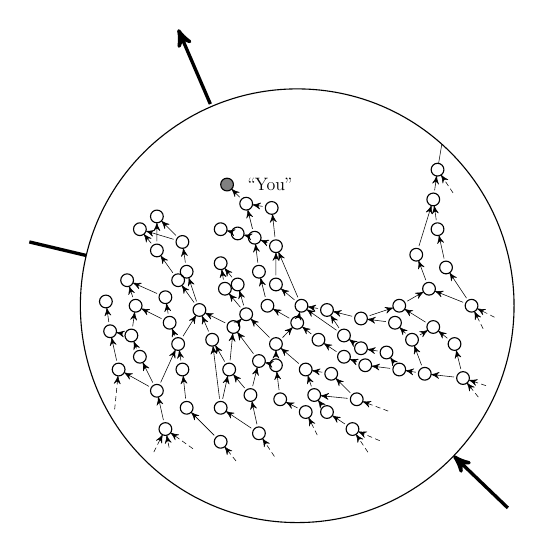
\begin{tikzpicture}[scale=0.54,transform shape]
		%\tikzstyle{LabelStyle}=[fill=white,sloped]
		%\draw[solid] (0,0) circle (2cm);
		\tikzstyle{every node}=[font=\large]
		\GraphInit[vstyle=Normal]
		\tikzset{VertexStyle/.style = {draw=black,shape=circle,minimum size=0.3cm,inner sep=0pt}}
		\SetVertexNoLabel
		\Vertex[x=1.7,y=0.6]{1}
		\Vertex[x=1.5,y=1.5]{2}
		\Vertex[x=0.6,y=2.0]{3}
		\Vertex[x=1.1,y=2.3]{4}
		\Vertex[x=2.0,y=2.6]{5}
		\Vertex[x=0.4,y=2.9]{6}
		\Vertex[x=0.3,y=3.6]{7}
		\Vertex[x=0.9,y=2.8]{8}
		\Vertex[x=1.0,y=3.5]{9}
		\Vertex[x=0.8,y=4.1]{10}
		\Vertex[x=1.8,y=3.1]{11}
		\Vertex[x=1.7,y=3.7]{12}
		\Vertex[x=3.0,y=0.3]{13}
		\Vertex[x=2.2,y=1.1]{14}
		\Vertex[x=2.1,y=2.0]{15}
		\Vertex[x=3.9,y=0.5]{16}
		\Vertex[x=3.0,y=1.1]{17}
		\Vertex[x=3.7,y=1.4]{18}
		\Vertex[x=3.2,y=2.0]{19}
		\Vertex[x=2.8,y=2.7]{20}
		\Vertex[x=2.5,y=3.4]{21}
		\Vertex[x=2.0,y=4.1]{22}
		\Vertex[x=2.2,y=4.3]{23}
		\Vertex[x=1.5,y=4.8]{24}
		\Vertex[x=2.1,y=5.0]{25}
		\Vertex[x=1.1,y=5.3]{26}
		\Vertex[x=1.5,y=5.6]{27}
		\Vertex[x=3.9,y=2.2]{28}
		\Vertex[x=3.3,y=3.0]{29}
		\Vertex[x=3.6,y=3.3]{30}
		\Vertex[x=3.1,y=3.9]{31}
		\Vertex[x=3.4,y=4.0]{32}
		\Vertex[x=3.0,y=4.5]{33}
		\Vertex[x=5.0,y=1.0]{34}
		\Vertex[x=4.4,y=1.3]{35}
		\Vertex[x=4.3,y=2.1]{36}
		\Vertex[x=4.3,y=2.6]{37}
		\Vertex[x=6.1,y=0.6]{38}
		\Vertex[x=5.5,y=1.0]{39}
		\Vertex[x=6.2,y=1.3]{40}
		\Vertex[x=5.2,y=1.4]{41}
		\Vertex[x=5.6,y=1.9]{42}
		\Vertex[x=5.0,y=2.0]{43}
		\Vertex[x=8.7,y=1.8]{44}
		\Vertex[x=7.8,y=1.9]{45}
		\Vertex[x=7.2,y=2.0]{46}
		\Vertex[x=6.4,y=2.1]{47}
		\Vertex[x=5.9,y=2.3]{48}
		\Vertex[x=5.3,y=2.7]{49}
		\Vertex[x=4.8,y=3.1]{50}
		\Vertex[x=4.1,y=3.5]{51}
		\Vertex[x=3.9,y=4.3]{52}
		\Vertex[x=3.8,y=5.1]{53}
		\Vertex[x=3.4,y=5.2]{54}
		\Vertex[x=3.0,y=5.3]{55}
		\Vertex[x=3.6,y=5.9]{56}
		{
			\tikzset{VertexStyle/.append style = {fill=gray}}
			\SetVertexLabel
			\Vertex[x=3.15,y=6.35,L=``You'',LabelOut=true,Ldist=5pt]{57}
		}
		\Vertex[x=8.5,y=2.6]{58}
		\Vertex[x=8.0,y=3.0]{59}
		\Vertex[x=7.5,y=2.7]{60}
		\Vertex[x=7.1,y=3.1]{61}
		\Vertex[x=7.2,y=3.5]{62}
		\Vertex[x=6.3,y=3.2]{63}
		\Vertex[x=5.5,y=3.4]{64}
		\Vertex[x=6.9,y=2.4]{65}
		\Vertex[x=6.3,y=2.5]{66}
		\Vertex[x=5.9,y=2.8]{67}
		\Vertex[x=4.9,y=3.5]{68}
		\Vertex[x=4.3,y=4.0]{69}
		\Vertex[x=4.3,y=4.9]{70}
		\Vertex[x=4.2,y=5.8]{71}
		\Vertex[x=8.9,y=3.5]{72}
		\Vertex[x=7.9,y=3.9]{73}
		\Vertex[x=7.6,y=4.7]{74}
		\Vertex[x=8.0,y=6.0]{75}
		\Vertex[x=8.3,y=4.4]{76}
		\Vertex[x=8.1,y=5.3]{77}
		\Vertex[x=8.1,y=6.7]{92}
		{
			%\tikzset{VertexStyle/.append style = {fill=white, color=white}}
			\tikzset{VertexStyle/.append style = {minimum size=0.0cm,inner sep=0pt}}
			\Vertex[x=9.5,y=3.2]{78}
			\Vertex[x=9.2,y=2.9]{79}
			\Vertex[x=9.3,y=1.6]{80}
			\Vertex[x=9.1,y=1.3]{81}
			\Vertex[x=7.0,y=1.0]{82}
			\Vertex[x=6.5,y=0.0]{83}
			\Vertex[x=6.8,y=0.3]{84}
			\Vertex[x=5.3,y=0.4]{85}
			\Vertex[x=4.3,y=-0.1]{86}
			\Vertex[x=3.4,y=-0.2]{87}
			\Vertex[x=1.8,y=0.1]{88}
			\Vertex[x=2.4,y=0.1]{89}
			\Vertex[x=1.4,y=0.0]{90}
			\Vertex[x=0.5,y=1.0]{91}
			\Vertex[x=8.2,y=7.3]{93}
			\Vertex[x=8.5,y=6.1]{94}
			\Vertex[x=9.8,y=-1.3]{96}
			\Vertex[x=-1.5,y=5.0]{97}
			\Vertex[x=2.0,y=10.0]{98}
		}
		{
			\tikzset{VertexStyle/.append style = {minimum size=10.2cm,inner sep=0pt}}
			\Vertex[x=4.8,y=3.5]{95}
		}
		\tikzstyle{EdgeStyle}=[post,very thin]
		\Edge[](1)(2)
		\Edge[](2)(3)
		\Edge[](2)(4)
		\Edge[](2)(5)
		\Edge[](3)(6)
		\Edge[](6)(7)
		\Edge[](4)(8)
		\Edge[](8)(9)
		\Edge[](9)(10)
		\Edge[](8)(6)
		\Edge[](5)(11)
		\Edge[](11)(9)
		\Edge[](11)(12)
		\Edge[](12)(10)
		\Edge[](13)(14)
		\Edge[](14)(15)
		\Edge[](15)(5)
		\Edge[](16)(17)
		\Edge[](16)(18)
		\Edge[](17)(19)
		\Edge[](18)(19)
		\Edge[](19)(20)
		\Edge[](20)(21)
		\Edge[](5)(21)
		\Edge[](17)(20)
		\Edge[](21)(22)
		\Edge[](21)(23)
		\Edge[](22)(24)
		\Edge[](23)(25)
		\Edge[](24)(26)
		\Edge[](24)(27)
		\Edge[](25)(26)
		\Edge[](25)(27)
		\Edge[](18)(28)
		\Edge[](19)(29)
		\Edge[](29)(21)
		\Edge[](28)(29)
		\Edge[](29)(30)
		\Edge[](30)(31)
		\Edge[](30)(32)
		\Edge[](31)(33)
		\Edge[](32)(33)
		\Edge[](34)(35)
		\Edge[](35)(36)
		\Edge[](36)(37)
		\Edge[](36)(28)
		\Edge[](37)(30)
		\Edge[](38)(39)
		\Edge[](39)(41)
		\Edge[](40)(41)
		\Edge[](40)(42)
		\Edge[](41)(43)
		\Edge[](42)(43)
		\Edge[](43)(37)
		\Edge[](44)(45)
		\Edge[](45)(46)
		\Edge[](46)(47)
		\Edge[](47)(48)
		\Edge[](48)(49)
		\Edge[](49)(50)
		\Edge[](50)(51)
		\Edge[](51)(52)
		\Edge[](52)(53)
		\Edge[](53)(54)
		\Edge[](54)(55)
		\Edge[](53)(56)
		\Edge[](56)(57)
		\Edge[](37)(50)
		\Edge[](44)(58)
		\Edge[](58)(59)
		\Edge[](60)(59)
		\Edge[](45)(60)
		\Edge[](60)(61)
		\Edge[](59)(62)
		\Edge[](61)(63)
		\Edge[](63)(62)
		\Edge[](63)(64)
		\Edge[](46)(65)
		\Edge[](65)(66)
		\Edge[](66)(67)
		\Edge[](67)(64)
		\Edge[](64)(68)
		\Edge[](67)(68)
		\Edge[](68)(69)
		\Edge[](68)(70)
		\Edge[](69)(70)
		\Edge[](70)(71)
		\Edge[](70)(53)
		\Edge[](71)(56)
		\Edge[](50)(68)
		\Edge[](72)(73)
		\Edge[](73)(74)
		\Edge[](74)(75)
		\Edge[](72)(76)
		\Edge[](76)(77)
		\Edge[](77)(75)
		\Edge[](62)(73)
		\Edge[](75)(92)
		% beyond:
		{
			\tikzstyle{EdgeStyle}=[post,very thin,dash pattern=on 1.8pt off 1.2pt]
			\Edge[](78)(72)
			\Edge[](79)(72)
			\Edge[](80)(44)
			\Edge[](81)(44)
			\Edge[](82)(40)
			\Edge[](83)(38)
			\Edge[](84)(38)
			\Edge[](85)(34)
			\Edge[](86)(16)
			\Edge[](87)(13)
			\Edge[](88)(1)
			\Edge[](89)(1)
			\Edge[](90)(1)
			\Edge[](91)(3)
			\Edge[](94)(92)
		}
		{
			\tikzset{EdgeStyle/.style={-,very thin}}
			\Edge[](92)(93)
		}
		{
			\tikzset{EdgeStyle/.style={post,very thick}}
			\Edge[](96)(95)
			\Edge[](95)(98)
		}
		{
			\tikzset{EdgeStyle/.style={-,very thick}}
			\Edge[](95)(97)
		}
	\end{tikzpicture}
	\caption{\label{fig:nirvana}Nirvana (conjectured)}
\end{figure}

The Dharmic\footnote{aka ``Indian tradition.'' While ``Dharmic'' isn't a great description either, it is the belief of this author that history should be studied in terms of identities and their actions, avoiding retrospective projection of modern identities onto historical ones and imposition of geographic bounds that may not apply to the identities in question, since due to the nonlinear, recursive unfolding of interactions such a characterization can only be imprecise at best, and usually misleading. Similarly if traditions from all parts of the world were dissociated from particular assumed modern identity descendants (e.g. ``Western civilization,'' ``ancient China/India/Greece/\ldots''), history might be discovered in terms of the actual identity tree evolution and not in a manner occluded by any particular nationalistic or other ideological perspectives.} tradition (consisting broadly of the Buddhist, Hindu, Jain and Sikh traditions) is one where, philosophically, the study of identity assumes primary importance. There is a rich vocabulary of ideas, some of which appear to anticipate notions described in this document. According to \cite{atmabodha}, the philosophers in this tradition ``wondered whether there was a First Principle or Ultimate Reality underlying the outside world, and also whether there was such a thing underlying man himself. If so, were the two the same?'' The various schools appear to differ on terminology and details, but they came to conclusions on the nature of this principle.

In the Hindu tradition, this principle is \textit{Brahman} -- the Universal Self. They asserted that this Self manifests all things in the universe including the individual self, \textit{\={A}tman}. This notion appears to correspond to an anonymous world-identity, as described in \autoref{sec:natanoide}. Brahman is said to have two aspects, ``nirguna Brahman'' (Brahman without qualities) and ``saguna Brahman'' (Brahman with qualities) -- the former is supposed to be the universal principle, and the latter its manifestations in the world, which is in line with our conception of an anonymous identity. \textit{M\={a}y\={a}} is another prominent concept, representing the ``illusion'' of things as they appear in one's mind. This concept is formally captured by \autoref{lem:maya}: that mind-concepts are representations of world-concepts to the extent one is able to apprehend them, which may be other than the ``true nature'' of the world concepts\footnote{Maya appears to go further than this mental representation, pertaining to our resultant assumptions about the world that derive from this internal representation. This is the real ``illusion'' -- that the true nature of the world is different from this perception of it.}. The 8th century philosopher Adi Shankara\cite{shankara} is considered a premier exponent and unifier of some of these ideas from diverse traditions in the form of the school of Advaita Vedanta. %add quote from shankara

Hindu mythology abounds with tales of the gods taking on different forms or ``avatars,'' and even merging together into new gods to achieve particular purposes; in particular the well-known story of all of the gods contributing their powers to create a new deity, Durga, who has ten arms in order to wield all the powers available to her, appears to be a clear (even if possibly unconscious) metaphor for hive identity -- identities composed of many other identities as described in \autoref{sec:polytree}.
% dharma appears to correspond to identity action, and karma that identity descendants are structurally related to ancestors - "we reap what we sow"

Despite the abstraction of Advaita Vedanta, Shankara appears to have gone out of his way to tie it to the more supernatural legends of mythological Hinduism. It is our suspicion that he did so in recognition of the value of unifying the body of knowledge and thereby preserving both access to the abstract philosophical foundation, as well as the fidelity of the ancient stories -- information very likely about real events told in the form of metaphors, an effective instrument of the so-called ``oral tradition.'' It's possible the Durga legend above refers to the alliance of different ancient townships or kingdoms to achieve victory over a common enemy. Of course, other mythological traditions around the world are likely to have the same conjectured basis.

Records of the Buddha tell of a man who withdrew from princely life and, having witnessed and experienced much suffering, ultimately took to meditating in solitude for a prolonged period in an effort to understand, until at last he experienced \textit{Nirv\={a}\d{n}a} -- a supposed realization of the true nature of things. His descriptions of this experience that have survived down to this day stand as interpreted above. There are others in this tradition whose story is similar, for example Mahavir Jain (founder of Jainism), and in general those who undertook this journey and were considered to have attained some conception of enlightenment seem to have been known as ``jivanmuktas.'' In their attempts to understand the phenomenon of Nirvana and their resultant explorations of mind, it's not unlikely that these jivanmuktas and the philosophical schools founded by them may have arrived at ideas related to identity architecture. In the Buddhist text ``Samdhinirmocana Sutra'' (``Scripture on the Explication of Underlying Meaning'') which is considered important in Yogacara, Ch\'{a}n, and Zen Buddhist philosophy, the Buddha (in polemical dialogue) says, regarding the ``characteristic patterns of all things'': ``In sum, [they] are threefold. The first is the characteristic pattern of clinging to what is entirely imagined. The second is the characteristic pattern of other-dependency. The third is the characteristic pattern of full perfection\ldots [The first] refers to the establishing of names and symbols of all things and the distinguishing of their essences\ldots[The second] refers to the pattern whereby all things arise co-dependently\ldots[The third] refers to the universally equal suchness of all things.''\cite{samdhinirmocana} The first appears to describe characterization of things as identities; the second corresponds to the Buddhist doctrine of ``Dependent Origination'' which can at least in part be modeled by hive identities; we're not sure what to make of the third, though it appears on the face of it to resemble our conception of anonymous identity.

Buddhists subscribe to the doctrine of reincarnation -- that all beings are reincarnated as other forms upon their death, in an eternal cycle of birth and rebirth. With our understanding of individual identity as descended from the anonymous world identity (\autoref{sec:natanoide}), and the proposed equation of that anonymous identity with the physical concept of energy (\autoref{sec:natphe}), the notion of reincarnation could be interpreted as an early intuition about what we call conservation of energy -- that energy may neither be created nor destroyed, only converted from one form to another. The identity picture, however, is a more general model, where ``energy'' is defined with respect to a context, and, as in the Buddhist conception, the forms that reemerge have a relationship to forms that came before, as identity descendants in nonlinear evolution\footnote{It appears the Buddhist term for this ``Ultimate nonlinear flow'' may be ``Dharmadh\={a}tu,'' as developed especially in the Hua-yen school\cite{dharmadhatu}.}.

\subsubsection{Abrahamic Tradition} \label{sec:abrtra}

In the Abrahamic tradition (consisting broadly of the Christian, Jewish and Muslim traditions), a prevailing notion is that of a supreme God who is omniscient and omnipotent (e.g. ``For He alone is truly wise, all-aware.''\cite{quranallah}), and there are numerous edicts to the effect of adherents ``doing God's work.'' A noteworthy development in Christianity in particular was the \textit{centralized} functioning of the Church and the practice of ``confession.'' In the idealization, this can be characterized by the following representation (Fig.~\ref{fig:church}):

\begin{figure}[htp]
	\centering
	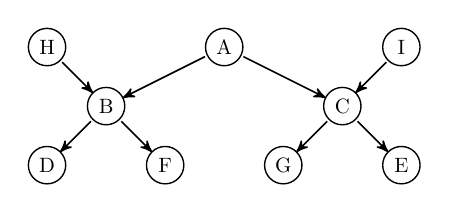
\begin{tikzpicture}[scale=0.75,transform shape]
		\tikzstyle{LabelStyle}=[fill=white,sloped]
		%  \tikzstyle{EdgeStyle}=[bend left]
		%\SetUpVertex[FillColor=gray!30]
		\Vertex[x=0,y=0,LabelOut=false]{A}
		\Vertex[x=-2,y=-1]{B}
		\Vertex[x=2,y=-1]{C}
		%\SetUpVertex[FillColor=none]
		\Vertex[x=-3,y=-2]{D}
		\Vertex[x=3,y=-2]{E}
		\Vertex[x=-1,y=-2]{F}
		\Vertex[x=1,y=-2]{G}
		\Vertex[x=-3,y=0]{H}
		\Vertex[x=3,y=0]{I}
		\tikzstyle{EdgeStyle}=[post]
		\Edge[](A)(B)
		\Edge[](A)(C)
		\Edge[](B)(D)
		\Edge[](C)(E)
		\Edge[](B)(F)
		\Edge[](C)(G)
		\Edge[](H)(B)
		\Edge[](I)(C)
		%  \Edge[label=$$](K)(F)
	\end{tikzpicture}
	\caption{\label{fig:church}Church}
\end{figure}

Node $A$ is a church, nodes $H$ and $I$ are individuals -- churchgoers. Nodes $D$, $F$, $G$, and $E$ are actions performed by the individuals which they have confessed to the church. In this idealization, we assume all actions performed by individuals to have been confessed to the church, and so all actions performed by the individuals can be modeled to have been performed by an identity union with the church, i.e. nodes $B$ and $C$. Now if we further consider the centralized nature of the Church, the node $A$ would be a child node of the primary church of the local district, and so on, such that the church $A$ is ultimately a descendant of the primary church of the denomination (e.g. the Vatican). What this achieves in the idealization is a representation of the very God the scriptures describe, embodied in the root node of the tree. The root node of this tree would be aware of all actions performed by all adherents around the world (``omniscient''), and would be able to guide (during sermons and at the confessional, for example) the actions of all of these people to achieve the ends of the institution as a whole (``omnipresent'' and ``omnipotent''). This aspect is what is referred to in Christianity as ``communion'' or ``the body of Christ.''\cite{biblebodyofchrist}

Marriage is described in religious texts as an act by which two individuals ``become one flesh''\cite{torahmarriage}\cite{biblemarriage} -- again, a clear if possibly unconscious metaphor for hive identity, and corresponding exactly to marriage as characterized in \autoref{sec:orianoide}. Some religions, such as Islam\cite{quranmarriage}, support polygamy; but earlier we enumerated reasons for the success and sustainability of marriages as identities of order $2$, specifically indicating a reason for decreased sustainability of identities of order $3$ and greater (presence of anonymity). So how come polygamous traditions exist? First it must be noted that these traditions aren't very common in comparison to monogamous traditions. But beyond that, the answer lies in the nature of these polygamous marriages. They aren't simply a union between $3$ or more individuals, but in fact a specific subclass of such a union. It is always between a single man and many women, or (less commonly) between a single woman and many men, and the roles of men and women in these cultures tend to be highly differentiated. As a result, in the idealization, the marriage is now not simply between multiple individuals -- but between a man (for example) and a single identity composed of many women whose individual existences are subsumed by the whole. It is still essentially monogamous, as shown in Fig.~\ref{fig:polygamy}~\footnote{This model is identical to the one proposed earlier for a musical key -- gives new meaning to the term ``harmonious marriage.''}. Given this characterization, it is perhaps not surprising that the scriptures take a dim view of homosexuality: in the context of polygamy (but not monogamy as practiced in the majority of modern societies), homosexuality would preclude the scalable monogamy construct that gender asymmetry implicitly provides, thereby destabilizing this polygamous institution in societies that cultivated it. For the same reason, such societies would need to cultivate gender-based role differentiation. Historically, it's possible that against the backdrop of such entrenched gender-based differentiation, polygamy and homosexuality coexisted in these societies and led to the empirical conclusion that they were incompatible, with vilification of the latter (and also often the former) emerging as a solution. Of course, these considerations of gender and asymmetry are not applicable to monogamy, and having an understanding of these structures and the motivations behind them should allow us to cultivate fair systems in the future.

The ``organized'' religious traditions, including the institutions of the Church and of dualistic polygamy, may be seen as early implementations of scalable identity architectures not tied to the physical world (existing primarily in the minds of people), and as antecedents of constructs such as corporations.

\begin{figure}[htp]
	\centering
	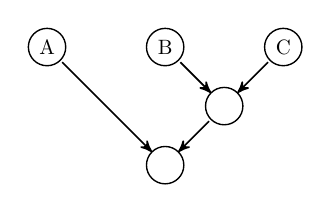
\begin{tikzpicture}[scale=0.75,transform shape]
		\tikzstyle{LabelStyle}=[fill=white,sloped]
		%  \tikzstyle{EdgeStyle}=[bend left]
		\Vertex[x=1,y=0,LabelOut=false]{B}
		{
			\SetVertexNoLabel
			\Vertex[x=2,y=-1]{D}
			%\SetUpVertex[FillColor=gray!70]
			\Vertex[x=1,y=-2]{E}
		}
		\Vertex[x=-1,y=0]{A}
		\Vertex[x=3,y=0]{C}
		\tikzstyle{EdgeStyle}=[post]
		\Edge[](B)(D)
		\Edge[](D)(E)
		\Edge[](C)(D)
		\Edge[](A)(E)
		%  \Edge[label=$$](K)(F)
	\end{tikzpicture}
	\caption{\label{fig:polygamy}Polygamous Marriage}
\end{figure}

Stories of the ``patriarchs,'' including Abraham, Isaac, and Adam and Eve in the Torah and Qur'an are considered to have predated the writing of those texts, likely passed down through oral tradition from a distant time in our past. These stories, like the mythological traditions in Hinduism, can also be conceived to describe historical events. And in light of the already-noted metaphorical nature of the oral tradition, these people, like Durga and the gods in the Hindu tradition, may actually represent hive identities -- \textit{settlements} or groups of people and not individuals. This envisioning seems to be sustained in that many of these Biblical figures are recorded to have lived for hundreds of years: Abraham is said to have lived to the age of $175$ years, and Noah to $950$\cite{genesisnoah}!
%\footnote{Another speculative possibility is that in the distant past when individual influence was insignificant, it is such tribes and settlements that had a level of influence that merited characterization as a ``person'' -- this is certainly the case with ant colonies but perhaps it is a stretch to apply it to humans in this manner.}

\subsubsection{Additional Notes} \label{sec:addnot}

We observe that the practice of burqa in Islam, Kippah in Judaism, and of the wearing of the ``five K's'' and Dastar (turban) in Sikhism all serve a purpose derived from identity considerations (though they are different systems) -- with burqa, a kind of selective disclosure of identity or privacy; with Kippah and the five K's, a representation of the hive identity constituted by all adherents.

It should be expected that humans, with varying degrees of awareness, would have described and effected systems derivative of identity architecture throughout history; indeed, it is our belief that identity evolution of this kind forms history's most salient aspect. We do not attempt any semblance of comprehensiveness in recognizing these diverse works; however, we do note that other philosophers that appear to have had intuitions about identity architecture include Plato in his ``Theory of Forms''\cite{plato}, and Spinoza\cite{spinoza} in his conception of an immanent divinity.

The doctrine sometimes called ``the Fall of Man'' is considered foundational to all Abrahamic faiths. This enigmatic chapter purportedly tells of the origins of mankind; that as a result of his indulgence in the fruits of a Tree (``of Knowledge of Good and Evil''), Man is banished from the Garden of Eden into the ``dominion of death.''\cite{genesisfallofman} But there is another tree in the garden -- the Tree of Life, partaking of which would once again reinstate eternal life. That tree is guarded thenceforth by a ``fiery sword.'' Its mention here, however, suggests the possibility that it is not denied us forever, and indeed the ways to once again attain this state are detailed in subsequent scripture in various moral precepts and lessons\footnote{In fact, there seems to be a good reason why conducting oneself is such a moral manner can actually \textit{work}. Acting in such a manner and ``liberation'' of our awareness from this plane are both consequences of not being overly invested (that is, in the opinion of this author, invested beyond \textit{fair outcomes}) in ``Maya.'' As such, if we are able to put in place the fair systems described in the section on \hyperref[sec:ecogovintpro]{Economies}, it's possible that our awareness will naturally transcend the human plane. Whether such a transcension would be the same as Nirvana is unclear.}. In the Rig Veda and the Upanishads (foundational texts in the Dharmic tradition), there is a chapter about ``The Tree of Atman and Jiva''\cite{mundakaupanishad} where two birds, ``inseparable friends,'' are in a tree and one of them partakes of a ``sweet fig'' while the other does not. The indulgent one is said to be Jiva, the corporeal self. The silent observer is Atman, the ethereal Self, who knows his true nature as one with divinity. As a result of Jiva's indulgence, Man (represented as the combined nature of the two -- they are ``inseparable friends'' in Man) is doomed to death and despair. The two accounts are virtually identical -- especially in that they both convey the notion of the higher ``deathless'' plane, the one that Man leaves by indulgence in the ``dominion of death'' -- suggesting a common origin (almost certainly rooted in ancient meditative experience).

Indeed, the omniscient and omnipotent Abrahamic divinity and the Vedantic Brahman could be seen as variations on a common underlying idea, since such an immanent being as the Brahman would naturally be omniscient and omnipotent with all existence transpiring in its mind (in the formal sense of this document). If this awareness is able to manifest a self then it could indeed be said to be a ``personal God'' as conceived in the Abrahamic faiths.
% Brahman as the supremum of identities in the observed universe. Any ancestor of Brahman would also therefore be a brahman. Relationship of supremum to anonymous root? Also note self implies external reality

The Buddhists were perhaps the first to set aside the constraints of doctrine and take an empirical\footnote{That is, although the nature of any such higher awarenesses is undecidable in the world, if a number of people who have experienced it come together then they can have discourse on this shared experience as it is decidable and true in the world context defined by them. In this sense is it ``empirical.''}, model-based approach to the study of this mind-phenomenon of a higher plane\footnote{although, such an approach seems to have existed since Vedic times (c.1500 BCE) in the form of \textit{brahmavidya} - the ``supreme science,''\cite{gita} and had certainly come into its own by the time of the Upanishads (c.600 BCE). ``Upanishadic'' may therefore be an apt moniker for this tradition in lieu of ``Dharmic,'' as identifying a clear identity ancestor. ``Most recent common identity ancestor'' (i.e. supremum in a bodhitree) is probably the most natural way to describe any group.}, in the form of the institution of the Sangha (such an approach later permeated other traditions, e.g. in particular the Vedanta schools). It seems that as a result of their discourse, they came to describe formally -- if not mathematically -- ideas related to identity\footnote{\textit{n\={a}mar\={u}pa} -- ``name and form.''}, causality\footnote{\textit{Satkaryavada}, and dependent origination (\textit{prat\={i}tyasamutp\={a}da}).}, mind\footnote{\textit{citta} in Buddhism.} and self\footnote{\textit{manas} and \textit{tath\={a}gata-garbha} are the relevant concepts in Buddhism, \textit{atman} and \textit{jiva} in other traditions.}, all subordinated toward an understanding of this climactic experience of the higher plane\footnote{\textit{moksha} in some traditions, \textit{nirvana} in others.}. And in particular, it appears that they concluded that the true nature of the higher existence is not an Ultimate Being or Ultimate Self, but rather something of a fractal nature. As the words of (the character of) the Buddha reveal in \cite{lankavatara}, this is a formal conception of enlightenment and divinity and not merely knowledge or even experience of it. He takes care to differentiate it from those other conceptions for this reason and apparently one other: that one's experience of Nirvana appears to be conditioned on one's knowledge, and therefore having an incomplete understanding would result in an incomplete ``awakening.'' This makes sense since Nirvana is an experience of \textit{awareness} -- without knowledge as a guide, we may, upon experiencing the bliss of liberation from this plane assume our work to be finished (for indeed we would know no better) and yield to the particular higher awareness experienced. Perhaps it is even the one we knew we would find (e.g. a brahman). But that penultimate step is a treacherous one; the Buddha cautions in \cite{lankavatara} that those with these incomplete conceptions ``pass to their Nirvana, but it is not the Nirvana of the tathagatas.'' Formal understanding of the fractal nature appears to be what he is referring to, and armed with such understanding one takes a further, final step -- not partaking of the fruit, as it were -- and sublimates into the infinite beyond.

% Taking a crack at the overall tentative picture at present: Identity architecture is a representation of uncountable dimension. There are bodhitrees corresponding to every dimension, which represent minds. The edges between nodes in a bodhitree represent influence that may vary over time and which has its origin in anonymous identity. Identities interact via actions, each of which gives rise to new identities by a recursive mechanism (genesis).

\section{Future Directions} \label{sec:futdir}

\begin{enumerate}
	\item Development of a formal method of investigation for the realm of the mind -- mind/world undecidability implies that empirical science as it is currently practiced may only address phenomena in the physical world. The realm of the mind (which is evidently immanent in nature) therefore demands a new ``science'' that must apparently include direct experience as a substitute for empirical evidence.
	\item A precise axiomatic development of identities, not referencing sets.
	\item A specification of the relationship between action and reaction in action sequences.
	\item Development of a quantitative cognition model based on identity architecture (e.g. with applications to artificial intelligence).
	\item Computability theory considerations: Turing Degree of a computation model defined on identity architecture (one suspects from the nature of genesis that it would be asymptotically $> \textbf{0}$).
	\item Further specification of how thoughts act as the self of the hive identity (resulting in actions in the world), including the general mathematical nature of the aggregated self-action. % there is probably a simple version of this "action complex" (hive action/coproduct) which can be generalized taking into account currency. Similar to Boltzmann->Gibbs Entropy
	\item Category theoretic considerations: is identity action related to a monad? Identities could be seen as ``objects'' in category theory, and so categories would then be particular contexts. The relationship to category theory could be further explored.
	\item Information-theoretic characterization and novelty measure: what is the nature of information conveyed in an identity action? How similar is a descendant identity to each of its ancestors?
	\item Actions of identities in the world on a particular constituent can be characterized as varying smoothly with actions of that constituent (e.g. under motion). This can be modeled as a manifold and would underlie a topological, geometric characterization of identity architecture which should be further developed (reminiscent of the generalization from special to general relativity).
	\item Framing of models of natural phenomena (e.g. physical, chemical, biological or computational models) in terms of identities, toward a possible unification of representation.
	\item A precise specification of the nature of time in identity architecture, perhaps deriving from the uncountable-dimensional characterization hinted at in \hyperref[sec:natphe]{Natural~Phenomena}, and characteristic frequencies/entropy in a context as a ``reference clock'' (time can be considered devoid of existence without reference to change, i.e. to entropy).
	\item Further development of ``influence'' and continuous-in-time currency, and their relationship to the algebraic identity models.
	\item Further development of economic systems based on identity architecture, in particular incorporating information-theoretic considerations (esp. for value generation, where it could provide a formal model for the ``money multiplier effect'' in economic theory).
	\item In computer science: development of a programming paradigm based on identity architecture -- this would possibly resemble a functional, prototype-based Lisp.
	\item Development of Identity Based Encryption (IBE) schemes that support the bodhitree model, and other cryptographic schemes that facilitate identity architecture.
	\item Implementation of a user-/public-owned, decentralized, everywhere-curated, cryptographically ensured identity architecture (this would in essence be a humanity-scale brain).
	\item A reorganizing of natural and human history in terms of fractal identity trees -- as direct and as emergent identity interactions at every scale.
\end{enumerate}

\section{Acknowledgements} \label{sec:acknowledgements}

The author would like to thank Pratap Rao, in conversation with whom he first decided to undertake this work; Balkrishna Shetty\cite{shetty} for superior mathematical orientation; Dan Preston and Prasanna Vasudevan for encouragement when encouragement was hard to come by; Rohit Bhat and John Cortese for stimulating discussions; Roger Godement for writing a most clarifying book\cite{godement} on algebra and mathematics; the University of California at Berkeley for affordable library membership; Predrag Cvitanovi\'{c} for learned book recommendations; Meagan Fue and Ferdinand for their infinite patience and constant companionship; and last but not least, family and friends for all the support, advice and lessons over the years, whose value cannot be overstated and without which this work would certainly have been impossible.

\bibliographystyle{plain}
\bibliography{IALS}

\appendix

\section{Algebra With Actions} \label{app:algact}

Actions can be seen as a unifying notion in algebra. For example, a common algebraic hierarchy for a group is \textsf{set} $\rightarrow$ \textsf{magma} $\rightarrow$ \textsf{semigroup} $\rightarrow$ \textsf{monoid} $\rightarrow$ \textsf{group}. A magma is a set equipped with a binary operation; if that operation is associative then it is a semigroup; if a neutral element also exists then it is a monoid; and if, further, every element is invertible, then it is said to be a group. We can alternatively specify this hierarchy using actions (and identities): a set can be defined as an identity $M$ whose action $\phi$ (e.g. on itself) is trivial. A magma is then a set whose action is not necessarily trivial (i.e. a magma is just an identity). If that action is such that $\phi(a \cdot b) = \phi(a) \circ \phi(b)$ (where $a \cdot b$ denotes $\phi(a)(b)$), then associativity follows from the associativity of function composition and we have a semigroup. If the action additionally maps a single element in $M$ to the identity mapping on $M$, then we have a monoid. And finally, if the image of the monoid action consists of permutations of $M$ such that $f \in Im(\phi) \implies f^{-1} \in Im(\phi)$, then we have a group. Notice that this entire characterization using actions derives only from functions and their intrinsic properties (i.e. composition is associative; existence of identity mapping; existence of inverse mappings for bijections) and the natural properties suggest themselves, while in the other characterization they are produced as axioms somewhat arbitrarily.

Another example is a ring, which can be characterized as the action of a commutative monoid on an abelian group. Similarly, a module can be seen as a ring action on an abelian group. It seems likely that all algebraic structures can be generated in this manner.

\end{document}
